\documentclass[10pt,a4paper]{article}
\usepackage[margin=2.3cm,headheight=14pt]{geometry}
\usepackage{fontspec}
\setmainfont{Libertinus Serif}
\setsansfont{IBM Plex Sans}
\setmonofont[Scale=0.86]{IBM Plex Mono}
\usepackage{microtype,graphicx,booktabs,xltabular,xcolor,float,fvextra,caption,fancyhdr,titlesec,enumitem}
\usepackage{placeins}
\usepackage[numbers,sort&compress]{natbib}
\usepackage[colorlinks,linkcolor=teal!70!black,citecolor=teal!70!black,urlcolor=teal!70!black]{hyperref}
\newfloat{listing}{tbp}{lol}\floatname{listing}{Listing}
\captionsetup{font=small,labelfont=bf}
\renewcommand{\tabularxcolumn}[1]{>{\raggedright\arraybackslash}p{#1}}
\setlength{\tabcolsep}{4pt}
\setlength{\LTpre}{6pt}\setlength{\LTpost}{6pt}
\setlist{itemsep=2pt,topsep=4pt}
\titleformat{\section}{\sffamily\Large\bfseries\color{teal!55!black}}{\thesection}{0.8em}{}
\titleformat{\subsection}{\sffamily\large\bfseries}{\thesubsection}{0.7em}{}
\renewcommand{\floatpagefraction}{0.75}\renewcommand{\topfraction}{0.85}\renewcommand{\textfraction}{0.12}
\pagestyle{fancy}\fancyhf{}
\fancyhead[L]{\sffamily\footnotesize The Robot Science Assistant: technical report}
\fancyhead[R]{\sffamily\footnotesize\nouppercase{\leftmark}}
\fancyfoot[C]{\sffamily\footnotesize\thepage}
\renewcommand{\headrulewidth}{0.3pt}
\begin{document}
\begin{titlepage}
\sffamily
\vspace*{2.2cm}
\noindent{\color{teal!55!black}\rule{\linewidth}{1.2pt}}\par\vspace{0.6cm}
\noindent{\Huge\bfseries The Robot Science Assistant\par}\vspace{0.4cm}
{\Large From culture-level plans to verified robot motions,\\ reproducible derivations and auditable executions\par}\vspace{0.6cm}
\noindent{\color{teal!55!black}\rule{\linewidth}{1.2pt}}\par\vspace{1.0cm}
{\large Technical report on the RSA kernel, its languages and its evaluation\\ on Cell 01 of the LabAutomationTwin\par}
\vspace{1.4cm}
{\normalsize [Authors and affiliations]\par}
\vfill
{\small\rmfamily
\begin{tabular}{@{}ll@{}}
Generated & 2026-10-17, from the pipeline's outputs \\
Manifest & \texttt{a8a39851a44328aac152ee46629decd9} \\
         & \texttt{cddc691b1e8c2b835c422bba7cd32659} \\
Example & challenge--rescue experiment, design \texttt{c\_\allowbreak{}d85\_\allowbreak{}t48\_\allowbreak{}n1} \\
Status & research prototype; biology is a surrogate, quantities ILLUSTRATIVE (D016) \\
\end{tabular}\par}
\end{titlepage}
\pagenumbering{roman}
\tableofcontents
\clearpage
\pagenumbering{arabic}

\section{Executive summary}\label{sec:summary}

This report documents the robot science assistant (RSA): a kernel that lets a robotic laboratory carry out an experiment stated at the level of the cultures, explain what it does, prove that its robot motions realize the stated experiment, and leave a record that anyone can verify and re-execute. The assistant is developed on Cell 01, a two-arm robotic cell of a physics-based laboratory twin, with one example: a challenge–rescue organoid experiment derived for an information gain of 0.5 bit. The report describes the concepts, the languages, the knowledge, the execution system, the verification and the reproducibility machinery, and reports every result with its source file. All biological quantities come from the twin's surrogate culture model and are ILLUSTRATIVE.

\textbf{What the assistant is.} The RSA is a plan-based controller for a robotic laboratory, built in the tradition of CRAM and structured reactive controllers~\citep{mcdermott1991,beetz2001,beetz2010}. An experiment is written once as a plan over the cultures. The assistant derives everything below it: a design chosen by expected information gain, a partially ordered plan of laboratory action designators with contracts and failure handlers, a CRAM/RPL controller, the robot and device steps, and constraint-based motion specifications for Giskard~\citep{stelter2022}. While it executes, it keeps beliefs with provenance and freshness, checks constraints before and during every action, repairs or escalates failures, and writes a hash-chained audit entry for every lifecycle transition of every designator. After the run, a critic judges realization and validity separately, and the assistant answers competency questions about what it did and why, with the grounds of each answer.

\textbf{What was shown.} The table below collects the main results. Each row is computed from the outputs of the pipeline at the manifest \texttt{a8a39851a44328aa}; the section given in the last column explains how.

\begin{table}[tbp]\centering\small
\caption{Main results of the RSA on the challenge–rescue example.}\label{tab:key}
\begin{tabularx}{\linewidth}{XXp{3.2cm}}\toprule
\textbf{Result} & \textbf{Value} & \textbf{Section} \\\midrule
Culture plan → lab plan → steps → motions & 12 → 8 → 151 → 111 & Section~\ref{sec:culture}, Section~\ref{sec:motion} \\
Expected / realized information gain & 0.5439 / 0.357 bit (required 0.5) & Section~\ref{sec:design}, Section~\ref{sec:culture} \\
Kernel run vs planner (nominal) & 153 leaves, identical step for step; 498 audit entries & Section~\ref{sec:exec} \\
Symbolic scenarios ending as specified & 12/12 & Section~\ref{sec:exec} \\
Isaac Sim runs ending as specified & 2/3 (calibration lapsed fails: F17) & Section~\ref{sec:isaac} \\
Competency-question checks & 52/52 correct, all grounded & Section~\ref{sec:audit} \\
LDL negative controls caught & 12/12 & Section~\ref{sec:ldl} \\
Handler guarantees verified & 13/13 & Section~\ref{sec:trust} \\
Refinement proof & QED relative to A1–A6; O1–O7 hold & Section~\ref{sec:proof} \\
Lab variants with identical culture plan & 13/13 & Section~\ref{sec:indep} \\
Reproduction of the derivation & 47/47 outputs identical; manifest \texttt{a8a39851a44328aa} & Section~\ref{sec:repro} \\
Audit trails & 15 intact, 15 tamper tests caught, 12/12 re-executions identical & Section~\ref{sec:repro} \\\bottomrule
\end{tabularx}
\end{table}

\textbf{What was not shown.} The assistant has not run in a wet laboratory. The culture is a surrogate model of the twin. Reproduction was checked on one machine. The Isaac Sim runs are recorded, not re-executed, and one of them does not end as specified; the cause (plate seating on the imager stage) is diagnosed but not repaired. The refinement proof is relative to six assumptions, two of which cover faults that the cell can detect only partly. The coraplex framework, the intended execution platform, was not yet installed; the kernel is shaped so that the port is a mapping, not a rewrite (Section~\ref{sec:roadmap}).

\textbf{How to read the report.} Section~\ref{sec:background} sets the scope and Section~\ref{sec:arch} the architecture. Section~\ref{sec:kb}–Section~\ref{sec:trust} describe the knowledge, the design, the lab designator language and the process models. Section~\ref{sec:culture}–Section~\ref{sec:motion} follow the experiment from the culture plan to robot motions and executions. Section~\ref{sec:proof}–Section~\ref{sec:repro} cover proof, independence and reproducibility. Section~\ref{sec:findings}–Section~\ref{sec:roadmap} list what the iterations taught, the limits and the next steps.

\section{Background, scope and method}\label{sec:background}

Robotic laboratories can run experiments around the clock and record everything they do~\citep{king2009,williams2015,burger2020,abolhasani2023}. They are usually programmed at the level of devices: a liquid-handler method, a robot program, a scheduler script. Such a program fixes \emph{how} an experiment is executed in one laboratory but does not state \emph{what} it does to the material, so it cannot be checked against the scientific intent, and it must be rewritten when the laboratory changes. Reproducibility suffers in both directions~\citep{baker2016}: the intent is not recorded in a checkable form, and the record of what happened is not tied to the intent.

The RSA addresses this with three commitments. First, the experiment is stated at the level of the cultures, independent of the laboratory. Second, every level below is derived and checked against the level above, so that the robot's motions provably realize the stated experiment, or fail safely. Third, the derivation and the execution are both recorded so that they can be verified and reproduced by someone else, in the spirit of FAIR data and data-integrity guidance~\citep{wilkinson2016,fda2018}.

\subsection{A rational reconstruction}\label{sec:recon}

The kernel is a \emph{rational reconstruction} of earlier try-outs in the ResearchSpace material: many good ideas in mutually inconsistent forms (designator schemas, taxonomies, audit formats, verdict vocabularies). The kernel does not try to unify everything. It takes one example and keeps only what that example needs. For each concept it records where it comes from and what was changed (Table~\ref{tab:concepts}). It then tests whether the result \emph{flies}: does the example run end to end, leave an audit trail, and answer competency questions correctly? Each iteration ends with findings that change the kernel or the knowledge; the findings log is in Section~\ref{sec:findings}.

\subsection{Cell 01 and the laboratory twin}\label{sec:cell}

Cell 01 is a robotic cell of a laboratory twin built on Isaac Sim with an OpenUSD scene and a semantic digital twin (SDT) in OWL. Two robots serve it: R01, a Franka FR3 that moves plates between the incubator (L10) and a handover nest, and R02, a UR5e on a rail that carries plates between the handover nest, the liquid handler (L12) in its enclosure, and the bright-field imager (L17), and couples a plate tool (T01) from an automatic tool changer. Further stations are a quarantine nest (H4), a plate hotel (L09) and a QC reference station (L21). The devices act themselves: L10 presents a plate on a shuttle, L12 doses a well, L17 loads and images. Cell 01 changes are made only through an overlay composer, so the as-built scene is never edited.

\begin{figure}[tbp]\centering
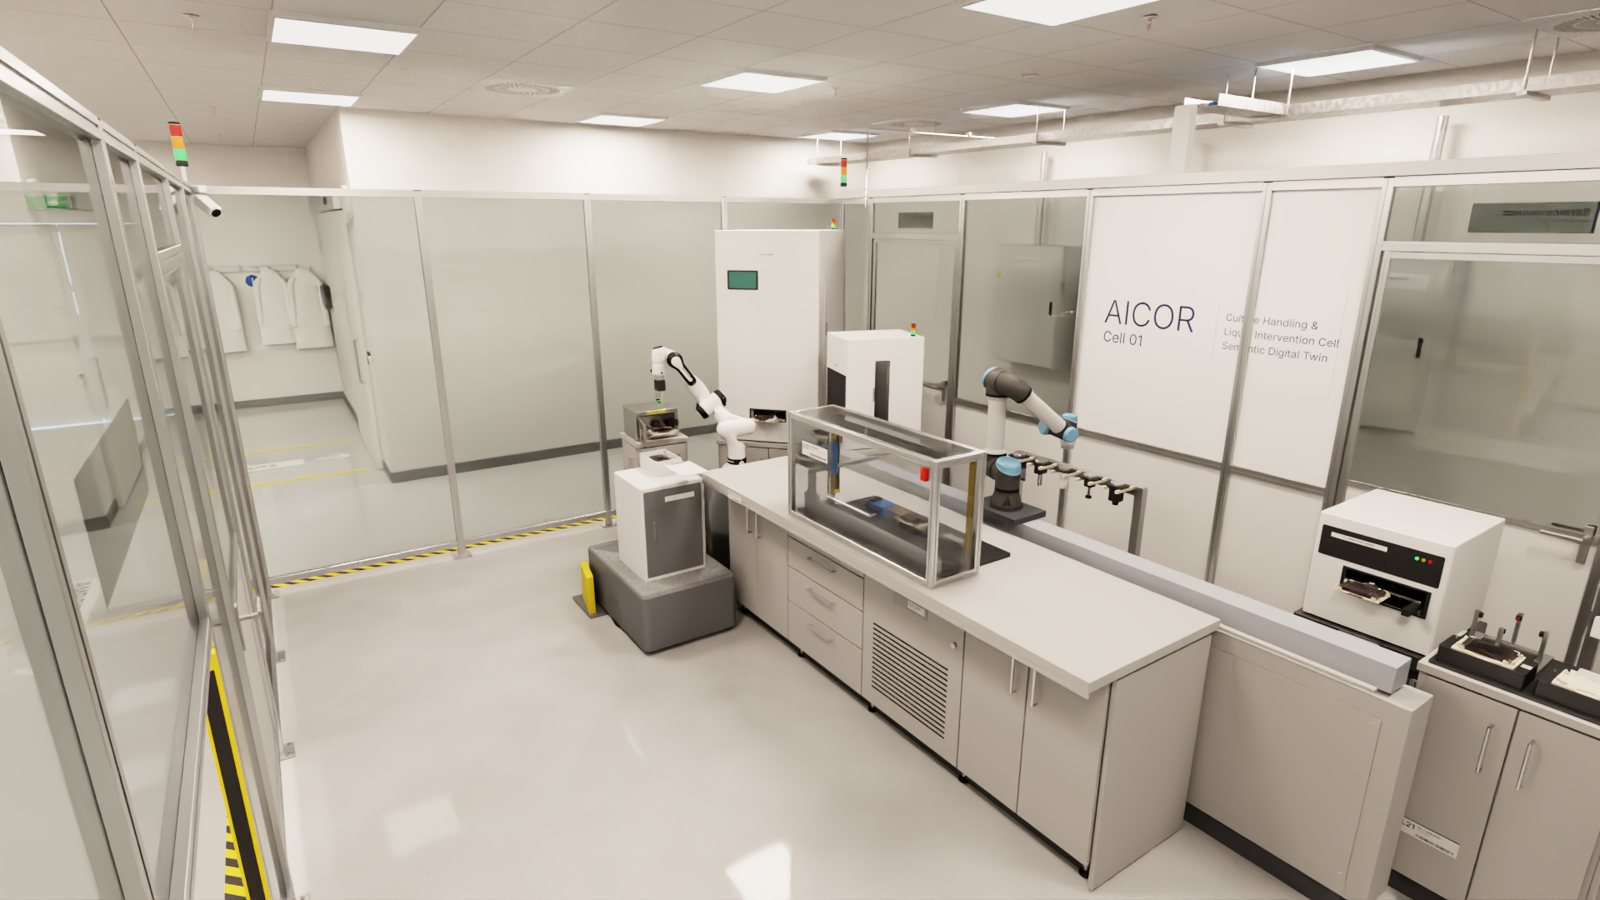
\includegraphics[width=\linewidth]{figures/cell.jpg}
\caption{Cell 01 in the laboratory twin (Isaac Sim, path-traced): two arms, the incubator, the liquid handler in its enclosure, the bright-field imager, the tool rack and the handover nest.}\label{fig:cell}
\end{figure}

\subsection{The example experiment}\label{sec:example}

The example is a challenge–rescue experiment on organoid cultures. Three competing recovery models (M1 graded, M2 threshold, M3 protective) predict different effects of a rescue given after a delay. The experiment challenges two cultures, rescues one of them after the delay, keeps a third culture untreated as control, images all three, and updates the belief over the models. The design is chosen to reach an expected information gain of at least 0.5 bit at least cost (Section~\ref{sec:design}). The selected design is \texttt{c\_\allowbreak{}d85\_\allowbreak{}t48\_\allowbreak{}n1}: challenge 0.85 au at 0 h into the rescued and the comparator culture, rescue 0.7 au at 48 h, images at 72 h. It runs in three sessions on plate P17, wells A01 (rescued), A02 (comparator) and A05 (control).

\textbf{ILLUSTRATIVE values (D016).} The culture is the twin's surrogate model; doses are in arbitrary units (au); the 600 s window outside the incubator, the 5 \% dose tolerance, KPI targets and the regulation mapping are twin values. They are labelled where they appear and are not asserted as laboratory or biomedical facts.

\subsection{Method: iterate on one example}\label{sec:method}

\begin{itemize}
  \item \textbf{Iteration 1} built the kernel and ran the example on a symbolic backend with fault injection: 12 scenarios, audit, critic, 27 competency questions (52 checks).
  \item \textbf{Iteration 2} added the Isaac Sim backend (same plan code) and expressed the kernel's categories as an OWL module checked by HermiT and Konclude.
  \item \textbf{Iteration 3a} introduced the lab designator language (LDL) in three versions (v0.1–v0.3), each after a round of design decisions, then the culture-level plan, its grounding in Cell 01, the Giskard motion level, the independence check, the refinement proof, and the reproducibility machinery.
  \item \textbf{Iteration 3 (pending)} ports the kernel to coraplex.
\end{itemize}

\section{Architecture}\label{sec:arch}

The assistant is organised in levels (Table~\ref{tab:levels}). Each level states something different, in its own language, and is derived from the level above. The culture plan is written; everything else is generated and checked.

\begin{table}[tbp]\centering\small
\caption{The levels of the RSA, from the culture plan to robot motions.}\label{tab:levels}
\begin{tabularx}{\linewidth}{lXlll}\toprule
\textbf{Level} & \textbf{States} & \textbf{Language} & \textbf{Derived by} & \textbf{Size} \\\midrule
Culture plan & what is done to the cultures, what becomes known & LDL (entity designators) & written & 12 actions \\
Design & doses, delay, replicates & EIG + ASP & nested Monte Carlo, clingo & 45 candidates \\
Lab plan & action designators with contracts and handlers & LDL & mapping, checked & 8 actions \\
Controller & structured reactive controller & CRAM/RPL (Lisp) & generated & 409 lines \\
Step plan & robot motions and device commands & kernel designators & clingo; kernel expansion & 151 steps \\
Motion plan & frames, constraints, monitors, cancels & giskardpy statecharts & generated & 111 motions \\\bottomrule
\end{tabularx}
\end{table}

Inside the kernel, seven components cooperate (Fig.~\ref{fig:arch}). The knowledge base answers resolution queries with their grounds. The plan library builds sub-plans of each action category at perform time. The executive drives designators through their lifecycle, projects plans before anything moves, applies the understanding gate and the policies, and handles failures. A backend executes leaves: a symbolic world with fault injection, or the Isaac Sim twin. Every transition goes into the audit trail, from which the critic and the competency-question engine work.

\begin{figure}[tbp]\centering
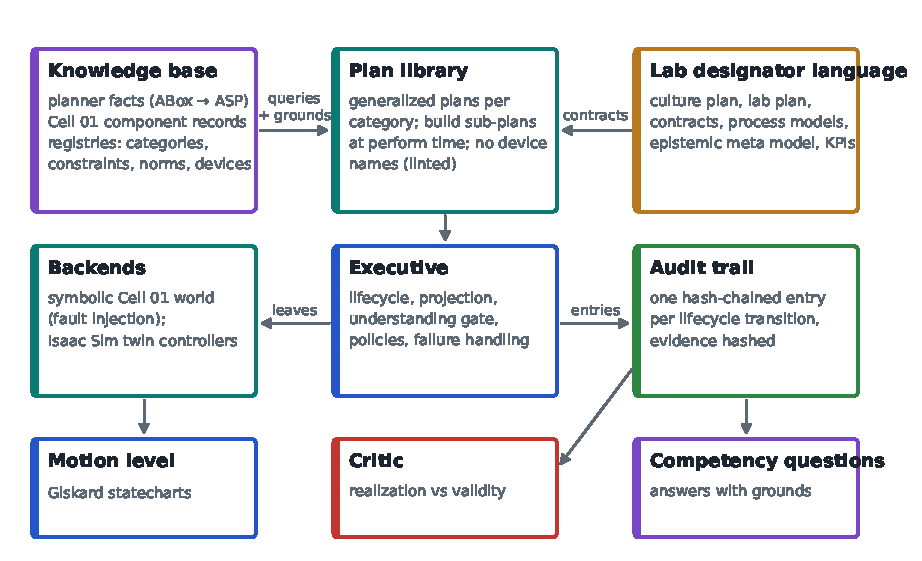
\includegraphics[width=0.95\linewidth]{figures/arch.pdf}
\caption{Kernel components and their data flow. The plan code never names a device; devices enter only through resolution against the knowledge base.}\label{fig:arch}
\end{figure}

\subsection{Twelve kernel concepts}\label{sec:concepts}

Table~\ref{tab:concepts} lists the twelve concepts the example needs, each with its kernel definition and origin. Three of them are new relative to the sources. The \emph{device-command designator} is a fourth leaf kind beside motions, because Cell 01's devices are co-actors. The \emph{event designator} is the audit-side record of what happened. And \emph{freshness} is part of belief, not only provenance (finding F2).

\begin{table}[tbp]\centering\small
\caption{The twelve kernel concepts, their definitions and where they come from.}\label{tab:concepts}
\begin{tabularx}{\linewidth}{lp{2.6cm}Xp{3.1cm}}\toprule
\textbf{\#} & \textbf{Concept} & \textbf{Kernel definition} & \textbf{Taken from} \\\midrule
1 & Designator & kind, category, determiner, bindings, constraints; kinds action, object, location, motion, device-command, event & HADL; KnowRob; coraplex \\
2 & Action category & a card owned by the category: level, parent, effect class, facet, roles, capability, pre/effects, sub-plan, monitors, recovery, evidence & KnowRob; Cell 01 schemas \\
3 & Category hierarchy & scientific → lab task → manipulation → motion, device-command beside motion; typed by effect class and facet & AICOR effect partition; Cell 01 \\
4 & Generalized plan & code of a category that builds the sub-plan from a bound designator at perform time, querying the knowledge base & CRAM; coraplex \\
5 & Resolution & a query returns value, grounds (fact atoms used) and rejected alternatives with reasons & KnowRob resolution; certificates \\
6 & Knowledge base & the planner's facts, the Cell 01 component records and the kernel registries; one source for all consumers & e2m derivation; Cell 01 SDT \\
7 & Capability & a verb qualified by state and by measurement binding (no match ⊂ capability match ⊂ provisional ⊂ validated) & Cell 01; RSV binding lattice \\
8 & Constraint & registry entry: id, column (realization or validity), source, text, applies-to, check, ASP rule, z3 theorem & uc\_\allowbreak{}ccr; e2m S1–S9 \\
9 & Lifecycle & open → grounded → accepted → executing → executed | failed → repaired | abstained | escalated & Cell 01 schemas \\
10 & Commitment record & one hash-chained entry per lifecycle transition, with bindings, grounds, verdicts, monitors and evidence & uc\_\allowbreak{}ccr audit; NEEM schema \\
11 & Two-column verdict & realization (ran correctly and safely) ⟂ validity (result interpretable); commit only if both hold & uc\_\allowbreak{}ccr critic \\
12 & Understanding gate + CQs & an incomplete understanding frame is not accepted; competency questions answered from the runtime trail & Cell 01 understanding contract \\\bottomrule
\end{tabularx}
\end{table}

\subsection{Code map}\label{sec:files}

The kernel is a Python package (\texttt{rsa/}) of about 7,580 lines. Its API is shaped like coraplex: designators are dataclasses, action designators build their plans, and plans are trees of sequential, try-in-order and monitor nodes with action, motion and command leaves.

\begin{table}[tbp]\centering\small
\caption{Modules of the RSA kernel and pipeline.}\label{tab:files}
\begin{tabularx}{\linewidth}{p{3.6cm}rX}\toprule
\textbf{Module} & \textbf{Lines} & \textbf{Role} \\\midrule
\texttt{rsa/kb.py} & 260 & knowledge base: planner facts, component records, registries; queries return grounds \\
\texttt{rsa/core.py} & 420 & designators, plan nodes, belief with provenance and freshness, executor \\
\texttt{rsa/library.py} & 405 & generalized plans of the categories; no device names (linted) \\
\texttt{rsa/checks.py} & 213 & constraint checks, policies (window, airspace), understanding frame \\
\texttt{rsa/backend.py} & 390 & symbolic Cell 01 world with fault injection \\
\texttt{rsa/isaac.py} & 558 & Isaac Sim backend: leaves bound to the twin's controllers \\
\texttt{rsa/audit.py} & 86 & hash-chained commitment records and verifier \\
\texttt{rsa/critic.py} & 92 & two-column verdict from the trail alone \\
\texttt{rsa/cq.py} & 436 & competency questions answered from trail, knowledge and dry runs \\
\texttt{rsa/ldl.py} & 839 & LDL parser, checker: order, threats, instruments, handlers, trust, KPIs \\
\texttt{rsa/ldl\_\allowbreak{}trust.py} & 452 & process models, guarantees, epistemic meta model \\
\texttt{rsa/ldl\_\allowbreak{}to\_\allowbreak{}cram.py} & 319 & CRAM/RPL controller generation \\
\texttt{rsa/culture\_\allowbreak{}plan.py} & 361 & culture plan: order, surrogate execution, mapping, feasibility \\
\texttt{rsa/grounding.py} & 260 & instantiation, trips, waits, computations, reactions \\
\texttt{rsa/motion\_\allowbreak{}frames.py} & 210 & goal frames from the scene; inverse kinematics reachability \\
\texttt{rsa/giskard\_\allowbreak{}motions.py} & 473 & Giskard motion statecharts \\
\texttt{rsa/refinement\_\allowbreak{}proof.py} & 269 & refinement proof O1–O7 and negative controls \\
\texttt{rsa/independence.py} & 230 & culture plan in 13 lab variants \\
\texttt{rsa/reproduce.py} & 204 & content-addressed manifest; verify by re-run \\
\texttt{rsa/protocol.py} & 181 & experimentation plan and audit certificate \\\bottomrule
\end{tabularx}
\end{table}

\section{Knowledge, designators and constraints}\label{sec:kb}

\textbf{One source of knowledge.} The planner, the resolver, the monitors and the competency questions read the same facts. They are generated from the OKF ontology ABoxes of the lab (SDT, safety, experiments) into ASP facts (\texttt{build/e2m/facts\_\allowbreak{}<tag>.lp}), complemented by the Cell 01 component records (capabilities, contracts, monitors, failure modes; read-only) and the kernel registries (categories, constraints, norms, devices, scenarios, competency questions). Two derivations from the same facts, the clingo plan and the kernel's expansion, must agree; they do, step for step (Section~\ref{sec:exec}).

\textbf{Resolution with grounds.} A resolution query returns a value, the fact atoms it used, and the alternatives it rejected with the reason. For the dosing step, the instrument resolves to L12's plate nest with grounds \texttt{has\_\allowbreak{}function(l12,dispensing)}, \texttt{dose\_\allowbreak{}well} among L12's capabilities and \texttt{seat(l12, …)}; five other devices are rejected, each with the missing function or capability. These records go into the audit trail, so the assistant can later answer why it chose a device.

\textbf{Designator lifecycle.} Each designator moves through the lifecycle of Fig.~\ref{fig:lifecycle}. Plan-node status (created, running, succeeded, failed), designator lifecycle and episode verdict are three separate vocabularies (decision K5); conflating them was a source of inconsistency in the earlier material.

\begin{figure}[tbp]\centering
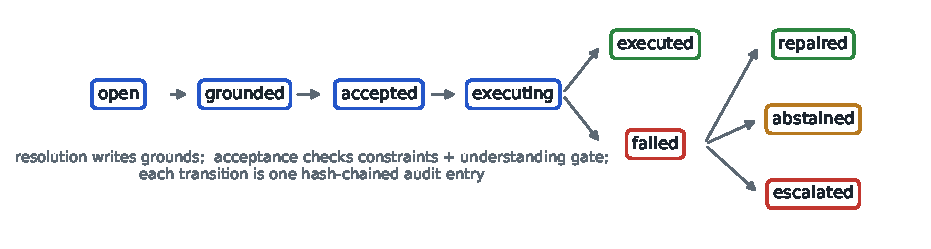
\includegraphics[width=\linewidth]{figures/lifecycle.pdf}
\caption{Designator lifecycle. Every transition is one audit entry; repairs are recorded on the node that repaired.}\label{fig:lifecycle}
\end{figure}

\subsection{Action categories}\label{sec:categories}

The category registry has 43 cards on five levels (Table~\ref{tab:categories}). A card belongs to the category, not to the instance: level, specialisation parent, refinement parts, effect class (the AICOR partition: object displacement, substance manipulation, perception, connecting, configuration change, regulation, maintenance), facet (transport, operation, transformation), roles, required capability, pre- and post-conditions as constraint ids, sub-plan, monitors, recovery and evidence obligations. The instance only binds roles. Expressed as an OWL module, the cards first produced six unsatisfiable classes, because \texttt{parent} mixed specialisation, partonomy and realisation (F14); separating \texttt{parent} from \texttt{parts} made the module consistent.

\begin{table}[tbp]\centering\small
\caption{Action categories by level (kernel registry).}\label{tab:categories}
\begin{tabularx}{\linewidth}{lrX}\toprule
\textbf{Level} & \textbf{\#} & \textbf{Categories} \\\midrule
scientific & 4 & \texttt{experiment}, \texttt{wait}, \texttt{intervene}, \texttt{measure} \\
lab task & 8 & \texttt{run\_\allowbreak{}session}, \texttt{retrieve}, \texttt{store}, \texttt{transport\_\allowbreak{}lab}, \texttt{dose}, \texttt{image}, \texttt{calibrate}, \texttt{quarantine} \\
manipulation & 6 & \texttt{transporting}, \texttt{picking\_\allowbreak{}up}, \texttt{placing}, \texttt{coupling\_\allowbreak{}tool}, \texttt{presenting}, \texttt{stowing} \\
device command & 16 & \texttt{check\_\allowbreak{}interlocks}, \texttt{verify\_\allowbreak{}identity}, \texttt{present}, \texttt{stow}, \texttt{wait\_\allowbreak{}environment}, \texttt{store\_\allowbreak{}cmd}, \texttt{tip\_\allowbreak{}pick}, \texttt{aspirate}, \texttt{dispense}, \texttt{tip\_\allowbreak{}eject}, \texttt{load}, \texttt{image\_\allowbreak{}well}, \texttt{autofocus}, \texttt{incubate}, \texttt{contain}, \texttt{validate} \\
motion & 9 & \texttt{approach}, \texttt{insert}, \texttt{grasp}, \texttt{lift}, \texttt{transit}, \texttt{place}, \texttt{release}, \texttt{retract}, \texttt{tool\_\allowbreak{}couple} \\\bottomrule
\end{tabularx}
\end{table}

\subsection{Constraints and norms}\label{sec:constraints}

Constraints are registry entries with a column. 14 runtime constraints guard the transitions of the categories they apply to; 7 validity checks (V1–V7) are evaluated by the critic over the whole episode (Table~\ref{tab:constraints}). Every constraint names its source: an ontology axiom, a Cell 01 monitor, an e2m axiom or a kernel finding.

{\footnotesize
\begin{xltabular}{\linewidth}{p{3.2cm}lp{1.9cm}Xp{3.0cm}}
\caption{Constraint registry: runtime constraints and the critic's validity checks.}\label{tab:constraints}\\
\toprule
\textbf{Constraint} & \textbf{Column} & \textbf{Applies to} & \textbf{Statement} & \textbf{Source} \\\midrule
\endfirsthead
\toprule
\textbf{Constraint} & \textbf{Column} & \textbf{Applies to} & \textbf{Statement} & \textbf{Source} \\\midrule
\endhead
\bottomrule
\endlastfoot
\texttt{interlocks\_\allowbreak{}closed} & realization & run\_\allowbreak{}session & enclosure interlocks are closed before a trip starts & safety.ofn enclosure\_\allowbreak{}door\_\allowbreak{}interlock; Cell 01 safety enclosure \\
\texttt{projection\_\allowbreak{}succeeds} & realization & experiment, run\_\allowbreak{}session & the plan can be projected to completion (every designator groundable) before anything is moved -- for the whole experiment before the first intervention, and again for each session before the plate leaves its home & CRAM projection / Ground \& Emulate gate (cram\_\allowbreak{}viz); kernel iteration … \\
\texttt{window\_\allowbreak{}prospective} & realization & run\_\allowbreak{}session & projected trip duration plus margin fits the window outside the incubator & e2m E2M8 S5 (600 s, 20 \% margin; ILLUSTRATIVE window) \\
\texttt{window\_\allowbreak{}kept} & realization & run\_\allowbreak{}session & elapsed time outside the incubator stays within the window & Cell 01 monitor time\_\allowbreak{}outside\_\allowbreak{}environment \\
\texttt{identity\_\allowbreak{}verified} & realization & retrieve & the plate identity read at the storage device matches the plate the session is about & safety.ofn identity\_\allowbreak{}verified; Cell 01 monitor plate\_\allowbreak{}identity \\
\texttt{environment\_\allowbreak{}before\_\allowbreak{}store} & realization & store & the incubator environment is accepted before the plate is stored & safety.ofn l10\_\allowbreak{}environment\_\allowbreak{}valid \\
\texttt{l12\_\allowbreak{}airspace\_\allowbreak{}clear} & realization & dose & no robot is in L12's deck airspace while L12 moves & safety.ofn l12\_\allowbreak{}deck\_\allowbreak{}airspace \\
\texttt{calibration\_\allowbreak{}before\_\allowbreak{}imaging} & realization & image & the imager is believed calibrated, or a QC calibration precedes the imaging & safety.ofn l17\_\allowbreak{}calibration\_\allowbreak{}valid \\
\texttt{tool\_\allowbreak{}compatible} & realization & coupling\_\allowbreak{}tool & a tool that contacts culture is compatible with the culture before coupling & Cell 01 contamination-and-asepsis \\
\texttt{contamination\_\allowbreak{}free} & realization & experiment, dose, transport\_\allowbreak{}lab & no challenge or rescue is performed on a plate under suspected contamination & safety rule contamination\_\allowbreak{}suspected\_\allowbreak{}blocks \\
\texttt{reagent\_\allowbreak{}bound} & realization & dose & the reagent is bound to a rack position with identity and lot before aspiration & Cell 01 L12 constraint 'Correct reagent identity/lot must be bound be… \\
\texttt{dispense\_\allowbreak{}completed} & realization & dose & dispense completed with the commanded volume within tolerance & Cell 01 monitor dispense\_\allowbreak{}completion; tolerance 5 \% ILLUSTRATIVE \\
\texttt{challenge\_\allowbreak{}requires\_\allowbreak{}controls} & validity & experiment & a challenge is authorised only if the design contains a control arm & safety rule challenge\_\allowbreak{}requires\_\allowbreak{}controls; uc\_\allowbreak{}ccr negative control (NR3) \\
\texttt{measurement\_\allowbreak{}binding\_\allowbreak{}validated} & validity & image & the imager's binding for the readout is validated (not only a capability match) & RSV measurement-binding lattice; VRB CF2 \\
\texttt{V1\_\allowbreak{}identity\_\allowbreak{}continuity} & validity & episode & every identity read in the run is the experiment's plate & Cell 01 critic identity; D009 \\
\texttt{V2\_\allowbreak{}calibration\_\allowbreak{}at\_\allowbreak{}measurement} & validity & episode & the imager was calibrated (observed) when each readout was acquired & Cell 01 monitor calibration\_\allowbreak{}state \\
\texttt{V3\_\allowbreak{}binding\_\allowbreak{}validated} & validity & episode & every readout comes from a validated measurement binding & RSV binding lattice \\
\texttt{V4\_\allowbreak{}controls\_\allowbreak{}present} & validity & episode & the control well was measured & uc\_\allowbreak{}ccr NR3 \\
\texttt{V5\_\allowbreak{}dose\_\allowbreak{}delivered} & validity & episode & each designed dose was delivered within tolerance (volume; not biological effective dose) & Cell 01 L12 'Executed volume is not equivalent to biological effectiv… \\
\texttt{V6\_\allowbreak{}sample\_\allowbreak{}integrity} & validity & episode & every trip kept the window outside the incubator & Cell 01 monitor time\_\allowbreak{}outside\_\allowbreak{}environment \\
\texttt{V7\_\allowbreak{}design\_\allowbreak{}realised} & validity & episode & every intervention and measurement of the design was executed at its designed culture time & e2m workflow (sessions) \\
\end{xltabular}}

Regulation clauses are cited by identifier only and mapped to what realises them in the kernel: an audit field, a runtime constraint, or a documentary obligation the kernel cannot discharge (Table~\ref{tab:norms}). The mapping is ILLUSTRATIVE. Its point is that the assistant can say which clauses a run covers and which it does not (competency question CQ-19).

\begin{table}[tbp]\centering\small
\caption{Regulation clauses and what realises them (ILLUSTRATIVE mapping).}\label{tab:norms}
\begin{tabularx}{\linewidth}{p{3.4cm}Xp{4.6cm}}\toprule
\textbf{Clause (ILLUSTRATIVE mapping)} & \textbf{Topic} & \textbf{Realised by} \\\midrule
EU-GMP-Annex11-9 & audit trail of GMP-relevant changes and actions & audit\_\allowbreak{}field: hash\_\allowbreak{}chain, lifecycle\_\allowbreak{}entry\_\allowbreak{}per\_\allowbreak{}transition \\
ALCOA-attributable & data attributable to who/what produced it & audit\_\allowbreak{}field: agent, software \\
ALCOA-contemporaneous & recorded when it happened & audit\_\allowbreak{}field: t\_\allowbreak{}sim \\
ALCOA-original & original record / true copy preserved & audit\_\allowbreak{}field: evidence\_\allowbreak{}sha256 \\
21CFR11-11.50 & signature manifestations (who, when, meaning) & documentary: quarantine\_\allowbreak{}release\_\allowbreak{}signoff \\
OECD-GLP-study-plan & study plan approved before the study starts & documentary: study\_\allowbreak{}plan\_\allowbreak{}approval \\
ISO10218-2-safeguarding & safeguarding of the robot cell & runtime: interlocks\_\allowbreak{}closed \\
biosafety-contamination & no handling of potentially contaminated cultures without containment & runtime: contamination\_\allowbreak{}free \\\bottomrule
\end{tabularx}
\end{table}

\subsection{Capabilities and measurement bindings}\label{sec:capability}

A capability is a verb from a component record, qualified by state (calibrated, tool coupled, tips present, automated) and by a measurement binding on a lattice: no match ⊂ capability match ⊂ provisional ⊂ validated. The distinction matters for validity. An imager that \emph{can} image a well but whose binding for the readout is not validated produces an image that does not count as evidence. This is how the \texttt{imager\_\allowbreak{}swapped} scenario ends realised but not valid (NR3), while \texttt{imager\_\allowbreak{}incapable} is refused before anything moves.

\section{Experimental design}\label{sec:design}

The design answers: which dose, delay and number of replicates separate the three recovery models best, at least cost? The assistant uses Bayesian experimental design~\citep{lindley1956,chaloner1995}: the expected information gain (EIG) of a design is the expected reduction of entropy of the belief over the models, estimated by nested Monte Carlo over the twin's calibrated surrogate. The planner then selects, among candidates meeting the required gain, the least-cost one that can be executed safely in Cell 01.

\begin{table}[tbp]\centering\small
\caption{The design problem and its solution.}\label{tab:design}
\begin{tabularx}{\linewidth}{p{3.6cm}X}\toprule
\textbf{Item} & \textbf{Value} \\\midrule
question & which recovery model (M1 graded, M2 threshold, M3 protective) explains the rescue efficacy after a delay \\
candidates evaluated & 45 (dose × delay × replicates); 13 meet the 0.5-bit requirement \\
EIG estimator & nested Monte Carlo, 800 samples, seed 7, uniform prior over 3 models (max 1.585 bit) \\
selected design & \texttt{c\_\allowbreak{}d85\_\allowbreak{}t48\_\allowbreak{}n1}: challenge 0.85 au, rescue 0.7 au after 48 h, 1 replicate \\
expected information gain & 0.5439 bit ≥ 0.5 bit \\
wells & rescued A01, comparator A02, control A05 \\
cost (least, then max EIG) & 9986 decisecond-equivalents (robot / device time + 60 s per well) \\
clingo & 332 atoms, 60750 rules, optimal \\\bottomrule
\end{tabularx}
\end{table}

\begin{figure}[tbp]\centering
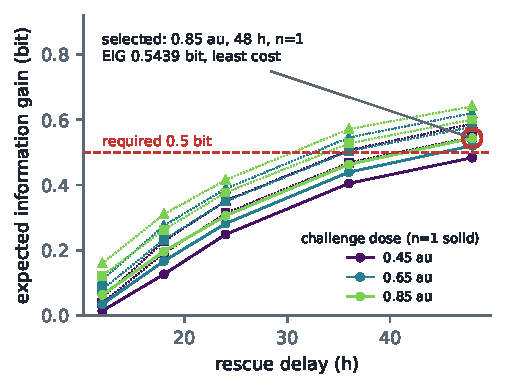
\includegraphics[width=0.62\linewidth]{figures/design.pdf}
\caption{Expected information gain of the candidate designs by delay and dose. The selected design is circled.}\label{fig:design}
\end{figure}

\subsection{From design to steps in ASP}\label{sec:asp}

The derivation from the selected design to the grounded steps is an answer-set program~\citep{gebser2019} that executes the experiment-to-motion axioms E2M1–E2M8. The stable model \emph{is} the plan: the selected experiment, the wells, the sessions, the trips, the routes and the ordered robot and device steps of every trip. Facts such as seats, shuttles, tools and durations come from the ontology; durations are apportioned from the twin's run traces. The excerpt in Listing~\ref{lst:asp} shows design selection, arm assignment with symmetry breaking, and the material of each session.

\begin{listing}[tbp]
\begin{Verbatim}[fontsize=\footnotesize,breaklines,frame=lines,framesep=2mm]
% ---------------------------------------------------------------------------------------------------- E2M1 selection
{ selected(C) : cand(C,_,_,_,G), req(Q), G >= Q } = 1.
sel(D,Dt,N,G) :- selected(C), cand(C,D,Dt,N,G).

% ---------------------------------------------------------------------------------------------------- E2M3 arms/units
{ role(W,rescued)    : free(W,_) } = N :- sel(_,_,N,_).
{ role(W,comparator) : free(W,_) } = N :- sel(_,_,N,_).
{ role(W,control)    : free(W,_) } = 1.
:- role(W,R1), role(W,R2), R1 != R2.
% symmetry breaking (wells are interchangeable units): the lowest free indices, rescued < comparator < control
used(W) :- role(W,_).
:- used(W2), free(W2,X2), free(W1,X1), X1 < X2, not used(W1).
rorder(rescued,1). rorder(comparator,2). rorder(control,3).
:- role(W1,R1), role(W2,R2), free(W1,X1), free(W2,X2), X1 < X2, rorder(R1,O1), rorder(R2,O2), O1 > O2.
treated(W) :- role(W,rescued).
treated(W) :- role(W,comparator).

% ---------------------------------------------------------------------------------------------------- E2M4 sessions
session(s0, 0).
session(s1, Dt) :- sel(_,Dt,_,_).
session(s2, 72).
mat(s0, dose(W,challenge,D)) :- sel(D,_,_,_), treated(W).
mat(s1, dose(W,rescue,R))    :- rescue_au(R), role(W,rescued).
mat(s2, image(W))            :- role(W,_).
kind(dose(W,X,Y), dose) :- mat(_, dose(W,X,Y)).
kind(image(W), image)   :- mat(_, image(W)).
well_of(dose(W,X,Y), W) :- mat(_, dose(W,X,Y)).
well_of(image(W), W)    :- mat(_, image(W)).
\end{Verbatim}
\caption{Excerpt of the experiment-to-motion axioms in ASP (selection, arms, sessions).}\label{lst:asp}
\end{listing}

\begin{table}[tbp]\centering\small
\caption{The three sessions of the derived plan, with planned and Isaac Sim durations.}\label{tab:sessions}
\begin{tabularx}{\linewidth}{lllXrrr}\toprule
\textbf{Session} & \textbf{Culture time} & \textbf{Device} & \textbf{Material} & \textbf{Steps} & \textbf{Planned (s)} & \textbf{Isaac (s)} \\\midrule
s0 & 0 h & L12 & dose A01 challenge 0.85 au; dose A02 challenge 0.85 au & 52 & 298.9 & 305.7 \\
s1 & 48 h & L12 & dose A01 rescue 0.70 au & 48 & 263.3 & 230.1 \\
s2 & 72 h & L17 & image A01; image A02; image A05 & 51 & 256.4 & 207.3 \\\bottomrule
\end{tabularx}
\end{table}

\subsection{SMT validation of the plan}\label{sec:z3}

An independent validator encodes the plan in z3~\citep{demoura2008} and proves the theorems V1–V5: executability and preservation of preconditions over all steps, safety rules, the time window with a ±20 \% duration tolerance, realization of the design (doses, images, session times), the arms with a control, the information gain, and least cost over all candidates meeting the requirement. 10 negative controls (mutated plans) are refuted. Finding F11 came from this layer: a QC calibration placed after the plate occupied the imager stage was physically infeasible in both derivations; the validator now refutes the old plan at step 24.

\begin{table}[tbp]\centering\small
\caption{SMT theorems over the derived plan (\texttt{validate\_\allowbreak{}plan\_\allowbreak{}z3.py}).}\label{tab:z3}
\begin{tabularx}{\linewidth}{XlX}\toprule
\textbf{Theorem} & \textbf{Holds} & \textbf{Detail} \\\midrule
V1 executability / preservation & yes & checked=278 \\
V2 safety S1 S2 S3 S6 S7 & yes & checked=115 \\
V3 time window (S5), durations +-20 \% & yes & checked=3 \\
V4 realisation (doses, images, session times) & yes & – \\
V4b arms E2M3 + control S9 & yes & – \\
V5 gain met (EIG >= g) & yes & eig\_\allowbreak{}bits=0.5439, required\_\allowbreak{}bits=0.5 \\
V5b least cost, then max EIG, over all candidates meeting g & yes & smt=unsat, compared=13 \\\bottomrule
\end{tabularx}
\end{table}

\section{The lab designator language}\label{sec:ldl}

The lab designator language (LDL) states \emph{what} a laboratory action must bring about, never \emph{how}. Every term is an entity description \texttt{(determiner sort slot*)} over lab entities only: plates, wells, substances, designs, arms, environments, excursions, transfers, measurements, records, instruments, persons and requests. A condition is an entity description too: once its variables are bound it is a ground query with a truth value. No robot, gripper, tool, pose, frame, trajectory or device identity can be written; a lint makes the boundary checkable.

\begin{table}[tbp]\centering\small
\caption{LDL clauses and their operational obligations.}\label{tab:ldl_clauses}
\begin{tabularx}{\linewidth}{lXX}\toprule
\textbf{Clause} & \textbf{Meaning over the action's interval} & \textbf{Operational obligation} \\\midrule
\texttt{requires} & holds (and is known to hold) at the start & acceptance check, or a reason to establish it first \\
\texttt{prevents} & no matching state or event occurs during the action & a detector and a reaction (abort, contain) \\
\texttt{maintains} & holds throughout the action & a regulator with a recorded history \\
\texttt{achieves} & holds at the end and persists until changed & post-condition with an evidence record \\
\texttt{goal} & the effect the action is for; links steps causally & justified by the experiment's goal \\
\texttt{signals} & the failures the action may raise & every failure needs a handler in the control program \\
\texttt{scope} & a non-terminating prevents/maintains opened and closed by fluents & a monitor around the realization \\\bottomrule
\end{tabularx}
\end{table}

\textbf{Semantics.} An execution trace satisfies an action iff its \texttt{requires} hold at the start, nothing its \texttt{prevents} describes occurs during the action, its \texttt{maintains} hold throughout, and its \texttt{achieves} hold at the end. \texttt{prevents} and \texttt{maintains} of an enclosing action are inherited by every sub-action; \texttt{achieves} is not. A condition φ marked \texttt{known} holds iff φ is believed with observed, fresh provenance; a plain \texttt{requires} may be established by the executive (insert a calibration), a \texttt{known} one may only be verified (identity cannot be established, only read). \textbf{Admissibility} sharpens the understanding gate: an action is accepted only if every term resolves, every \texttt{prevents} item has a monitor that can detect it, every \texttt{maintains} item a monitor or regulator, every \texttt{achieves} item an evidence path, and every \texttt{requires} item can be verified or established. A \texttt{prevents} clause that nothing can observe is not a constraint, so the action is refused.

\begin{listing}[tbp]
\begin{Verbatim}[fontsize=\footnotesize,breaklines,frame=lines,framesep=2mm]
(contract intervening
  (roles (into (the well ?w (of ?p))) (substance ?s) (dose ?q) (at (culture-time ?t)))
  (instrument (an instrument ?d
    (slot (a plate-slot (accepts ?p)))
    (process (a process (type substance-transfer) (into ?w) (of ?s) (amount ?q)))))
  (goal (the well ?w (received ?s ?q)) :tolerance 5 % :column validity)
  (requires
    (known (the plate ?p (identity verified))) :consequential
    (known (some substance ?s (identity verified))) :consequential
    (believed (the plate ?p (contamination none)) (grade (source inferred))) :consequential
    (the plate ?p (culture-time ?t)))
  (prevents
    (an event (type contamination-introduced) (of ?p)))
  (scope (begins-when (a portion ?u (of ?s) (drawn-for ?self)))
         (ends-when (the portion ?u (delivered true)))
    (prevents (a transfer (of ?u) (into (a well (of ?p) (not ?w))))))
  (achieves
    (a transfer (of ?s) (into ?w))
    (a record (of ?self) (states ?w ?s ?q ?t) (original true)))
  (signals
    (a failure (type identity-mismatch))
    (a failure (type dose-not-delivered))
    (a failure (type contamination-suspected))))
\end{Verbatim}
\caption{The contract of the action type \texttt{intervening} (\texttt{registry/lab/contracts.ldl}).}\label{lst:contract}
\end{listing}

\subsection{Instruments as roles}\label{sec:instruments}

Instruments appear only attributively, but they fill a role: a slot the plate is inserted into and a process that, once started, performs the action. Realization is machine tending: insert, start, await, remove. The checker resolves every role against the knowledge (Table~\ref{tab:instruments}): an automated device with a plate seat, with the function and capability verb of the process.

\begin{table}[tbp]\centering\footnotesize
\caption{Instrument roles of the lab plan and how they resolve in Cell 01.}\label{tab:instruments}
\begin{tabularx}{\linewidth}{llp{3.2cm}Xr}\toprule
\textbf{Step} & \textbf{Process} & \textbf{Function / capability} & \textbf{Device and slot} & \textbf{Rejected} \\\midrule
?x1 & substance-transfer & dispensing / \texttt{dose\_\allowbreak{}well} & L12 \texttt{stations\_\allowbreak{}l12\_\allowbreak{}liquidhandler\_\allowbreak{}plate\_\allowbreak{}nest} & 5 \\
?x2 & substance-transfer & dispensing / \texttt{dose\_\allowbreak{}well} & L12 \texttt{stations\_\allowbreak{}l12\_\allowbreak{}liquidhandler\_\allowbreak{}plate\_\allowbreak{}nest} & 5 \\
?w1 & incubation & incubation / \texttt{incubate\_\allowbreak{}plate} & L10 \texttt{stations\_\allowbreak{}l10\_\allowbreak{}incubator\_\allowbreak{}transfer\_\allowbreak{}station} & 5 \\
?x3 & substance-transfer & dispensing / \texttt{dose\_\allowbreak{}well} & L12 \texttt{stations\_\allowbreak{}l12\_\allowbreak{}liquidhandler\_\allowbreak{}plate\_\allowbreak{}nest} & 5 \\
?w2 & incubation & incubation / \texttt{incubate\_\allowbreak{}plate} & L10 \texttt{stations\_\allowbreak{}l10\_\allowbreak{}incubator\_\allowbreak{}transfer\_\allowbreak{}station} & 5 \\
?m1 & imaging & imaging / \texttt{image\_\allowbreak{}well} & L17 \texttt{stations\_\allowbreak{}l17\_\allowbreak{}brightfieldimager\_\allowbreak{}plate\_\allowbreak{}load\_\allowbreak{}frame} & 5 \\
?m2 & imaging & imaging / \texttt{image\_\allowbreak{}well} & L17 \texttt{stations\_\allowbreak{}l17\_\allowbreak{}brightfieldimager\_\allowbreak{}plate\_\allowbreak{}load\_\allowbreak{}frame} & 5 \\
?m3 & imaging & imaging / \texttt{image\_\allowbreak{}well} & L17 \texttt{stations\_\allowbreak{}l17\_\allowbreak{}brightfieldimager\_\allowbreak{}plate\_\allowbreak{}load\_\allowbreak{}frame} & 5 \\\bottomrule
\end{tabularx}
\end{table}

\subsection{Order, goals and threats}\label{sec:order}

The order of the lab plan is derived, not written. From goals and \texttt{achieves} the checker builds 13 causal links; 9 threats on culture time are all resolved by promotion, leaving 7 Hasse edges and 12 linear extensions, in the manner of least-commitment planning~\citep{weld1994}. Every step goal is justified by the experiment's goal through the links. A \texttt{scope} bounds a non-terminating prevents-item by fluents: the cross-dosing prevents-item holds only while the portion drawn for the action is in the tip, which removed a spurious mutual exclusion between dosing A01 and A02 that v0.1 produced.

\begin{listing}[tbp]
\begin{Verbatim}[fontsize=\footnotesize,breaklines,frame=lines,framesep=2mm]
(an action ?x3
    (type intervening)
    (into ?r)
    (substance ?rs)
    (dose 0.70 au)
    (at (culture-time 48 h)))
\end{Verbatim}
\caption{A lab action designator of the generated plan (the rescue dose).}\label{lst:lab}
\end{listing}

\subsection{Failures and handlers}\label{sec:handlers}

Each contract lists the failures it may signal. The experiment's control program handles them: \texttt{(on (a failure …) (do …) (then retry | replan | escalate) (else …) (guarantees …))}. All 21 signalled failures of the plan have a handler. Listing~\ref{lst:handlers} shows the handlers; Table~\ref{tab:handlers} in the appendix lists them all.

\begin{listing}[tbp]
\begin{Verbatim}[fontsize=\footnotesize,breaklines,frame=lines,framesep=2mm]
(handles                                             ; every handler states the guarantee it claims; rsa/ldl.py checks it
  (on (a failure (type identity-mismatch))
      (do (an action (type quarantining) (material (the plate (identity mismatched)))))
      (then escalate)
      (guarantees safe-state contained))
  (on (a failure (type measurement-invalid) (cause calibration_expired))
      (do (re-establish (an instrument (function imaging) (calibration current))))
      (then replan) (else escalate)
      (guarantees goal-or-safe-state))
  (on (a failure (type measurement-invalid) (cause out_of_focus))
      (do (re-establish (the plate ?p (seated true))))
      (then (retry (max 1))) (else escalate)
      (guarantees goal-or-safe-state))
  (on (a failure (type measurement-invalid) (cause plate_misseated))
      (do (re-establish (the plate ?p (seated true))))
      (then (retry (max 1))) (else escalate)
      (guarantees goal-or-safe-state))
  (on (a failure (type validity-effect-unachievable))
      (then escalate)
      (guarantees safe-state))
  (on (a failure (type dose-not-delivered) (cause wrong_reagent))
      (do (re-establish (some substance ?s (identity verified))))
\end{Verbatim}
\caption{Handlers of the experiment's control program (excerpt of \texttt{challenge\_\allowbreak{}rescue.ldl}).}\label{lst:handlers}
\end{listing}

\subsection{Negative controls}\label{sec:ldlneg}

A checker that accepts everything proves nothing. Each of the 12 mutations in Table~\ref{tab:ldlneg} breaks one property, and the checker must refuse it with the right reason.

\begin{table}[tbp]\centering\footnotesize
\caption{Negative controls of the LDL checker; each mutation must be caught.}\label{tab:ldlneg}
\begin{tabularx}{\linewidth}{p{5cm}X}\toprule
\textbf{Negative control (mutation)} & \textbf{Caught by} \\\midrule
N1 design anchors removed & ?w1 threatens start -> ?x1 ((the plate ?p (culture-time 0 h))); ?w2 threatens start -> ?x1 ((the plate ?p (culture-time… \\
N2 control well dosed & VIOLATED by ['?x9'] \\
N3 design without a control arm & ?k; VIOLATED \\
N4 device named in lab text & device or robot id 'l17' in (on l17) \\
N5 rescue at a culture time nothing achieves & ?x3: (the plate ?p (culture-time 36 h)) \\
N6 identity-mismatch handler removed & ?m1: identity-mismatch unhandled; ?m2: identity-mismatch unhandled \\
N7 instrument process no device offers & ?m1: ['h4', 'no device function realises process sequencing']; ?m2: ['h4', 'no device function realises process sequenc… \\
N8 a step whose goal serves nothing & ?m9 unjustified \\
N9 focus retry without re-seating (F17) & out\_\allowbreak{}of\_\allowbreak{}focus is persistent and the handler does not re-establish (the plate ?p (seated true)): a retry meets the same c… \\
N10 process fault not in the component record & L12\_\allowbreak{}LiquidHandler: ["fault pipette\_\allowbreak{}crash not in the record's failure\_\allowbreak{}modes"] unmodelled ['well\_\allowbreak{}misregistration'] \\
N11 repair claims the goal after the irreversible phase & well\_\allowbreak{}misregistration occurs at dispense, at or after the irreversible phase dispense; the goal cannot be re-achieved \\
N12 meta model without rules for weak consequential beliefs & (the plate ?p (identity verified)): ['inferred', 'assumed'] untreated \\\bottomrule
\end{tabularx}
\end{table}

\section{Process models, trust, guarantees and quality}\label{sec:trust}

The trustworthiness of an experiment depends on what happens \emph{inside} the devices. LDL v0.3 therefore models each laboratory process: its phases, the phase after which it cannot be undone, and its faults. Each fault states the failure it signals, the goal it corrupts, the monitor that detects it and with what coverage, whether a repeat meets the same cause (persistence), and which re-established condition removes it. The models are grounded in the Cell 01 component records: every fault must be one of the record's failure modes, every monitor one of its observations.

\begin{listing}[tbp]
\begin{Verbatim}[fontsize=\footnotesize,breaklines,frame=lines,framesep=2mm]
(process-model substance-transfer
  (realised-by (an instrument (function dispensing)))
  (component L12_LiquidHandler)
  (contract dose_well)
  (phases verify-reagent pick-tip aspirate dispense eject-tip)
  (irreversible-at dispense)
  (produces (the well ?w (received ?s ?q)))
  (faults
    (a fault (name wrong_reagent) (signals dose-not-delivered) (at verify-reagent)
      (corrupts (the well ?w (received ?s ?q)))
      (detected-by (a monitor (control "reagent identity check"))) (coverage full)
      (persistence persistent) (removed-by (some substance ?s (identity verified)))
      (record-recovery "abort before aspiration; quarantine if dispense occurred"))
    (a fault (name tip_missing_or_dropped) (signals dose-not-delivered) (at pick-tip)
      (corrupts (the well ?w (received ?s ?q)))
      (detected-by (a monitor (observation "tip-presence sensor"))) (coverage full)
      (persistence transient)
      (record-recovery "abort; replace tip; evaluate plate exposure"))
    (a fault (name clog_or_air_aspiration) (signals dose-not-delivered) (at aspirate)
      (corrupts (the well ?w (received ?s ?q)))
      (detected-by (a monitor (observation "pressure trace"))) (coverage full)
      (persistence transient)
      (record-recovery "mark dose uncertain; repeat only if protocol allows"))
    (a fault (name well_misregistration) (signals dose-not-delivered) (at dispense)
      (corrupts (the well ?w (received ?s ?q)))
      (detected-by (a monitor (observation "nest sensor + vision"))) (coverage partial)   ; sees a misseated plate, not the dispense position
      (persistence persistent) (removed-by (the plate ?p (seated true)))
      (record-recovery "quarantine affected plate; do not silently correct provenance")))
  (evidence "reagent lot" "tip ID/type" "volume" "pressure trace" "well identity")
  (must-not-assume "commanded volume equals delivered volume" "delivered dose equals biological injury"))
\end{Verbatim}
\caption{Process model of substance transfer (L12), \texttt{registry/lab/processes.ldl}.}\label{lst:process}
\end{listing}

\begin{table}[tbp]\centering\footnotesize
\caption{Process models and their grounding in the Cell 01 components.}\label{tab:models}
\begin{tabularx}{\linewidth}{lp{2.4cm}XlXX}\toprule
\textbf{Process} & \textbf{Component} & \textbf{Phases} & \textbf{Irreversible} & \textbf{Faults} & \textbf{Must not assume} \\\midrule
substance-transfer & L12\_\allowbreak{}LiquidHandler & verify-reagent → pick-tip → aspirate → dispense → eject-tip & dispense & wrong\_\allowbreak{}reagent, tip\_\allowbreak{}missing\_\allowbreak{}or\_\allowbreak{}dropped, clog\_\allowbreak{}or\_\allowbreak{}air\_\allowbreak{}aspiration, well\_\allowbreak{}misregistration & commanded volume equals delivered volume; delivered dose equals biological injury \\
imaging & L17\_\allowbreak{}BrightFieldImager & load → autofocus → acquire → assess → export & none & calibration\_\allowbreak{}expired, plate\_\allowbreak{}misseated, out\_\allowbreak{}of\_\allowbreak{}focus & morphology image directly equals biological state \\
incubation & L10\_\allowbreak{}Incubator & store → hold → release & hold & temperature\_\allowbreak{}excursion, CO2\_\allowbreak{}excursion, gate\_\allowbreak{}stuck\_\allowbreak{}open & nominal setpoint equals actual culture exposure without sensor evidence \\
containment & H4\_\allowbreak{}Quarantine & receive → isolate → hold & none & unauthorized\_\allowbreak{}release & quarantine implies biological failure \\\bottomrule
\end{tabularx}
\end{table}

\subsection{Trust per step}\label{sec:truststep}

Reasoning over the models gives the trust profile of each step (Fig.~\ref{fig:trust}, Table~\ref{tab:trust}). 21 of 27 fault occurrences are fully detected. Two fault kinds are only partly detected: well misregistration at L12, which occurs at the irreversible dispense, and plate misseating at L17, the lateral shift behind finding F17. They are the two trust gaps of the current cell and appear as assumption A2 of the refinement proof.

\begin{figure}[tbp]\centering
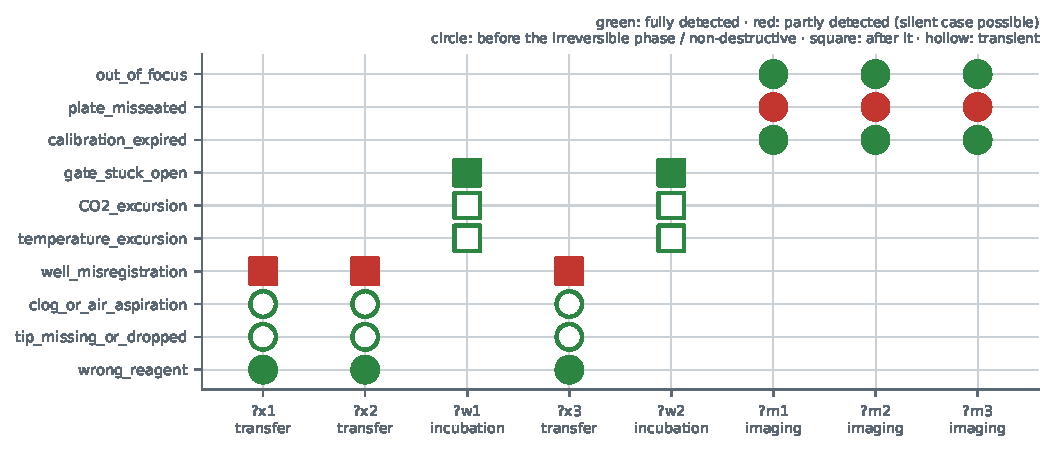
\includegraphics[width=\linewidth]{figures/trust.pdf}
\caption{Trust profile of the lab plan: fault × step, by detection coverage, timing relative to the irreversible phase, and persistence.}\label{fig:trust}
\end{figure}

\begin{table}[tbp]\centering\footnotesize
\caption{Faults of the process models: detection, timing, persistence and handling.}\label{tab:trust}
\begin{tabularx}{\linewidth}{p{3.2cm}lXllll}\toprule
\textbf{Fault} & \textbf{Process} & \textbf{Detected by} & \textbf{Coverage} & \textbf{Timing} & \textbf{Persistence} & \textbf{Handled} \\\midrule
\texttt{wrong\_\allowbreak{}reagent} & substance-transfer & reagent identity check & full & before the irreversible phase & persistent & yes \\
\texttt{tip\_\allowbreak{}missing\_\allowbreak{}or\_\allowbreak{}dropped} & substance-transfer & tip-presence sensor & full & before the irreversible phase & transient & yes \\
\texttt{clog\_\allowbreak{}or\_\allowbreak{}air\_\allowbreak{}aspiration} & substance-transfer & pressure trace & full & before the irreversible phase & transient & yes \\
\texttt{well\_\allowbreak{}misregistration} & substance-transfer & nest sensor + vision & partial & after the irreversible phase & persistent & yes \\
\texttt{temperature\_\allowbreak{}excursion} & incubation & temperature sensor & full & after the irreversible phase & transient & yes \\
\texttt{CO2\_\allowbreak{}excursion} & incubation & CO2 sensor & full & after the irreversible phase & transient & yes \\
\texttt{gate\_\allowbreak{}stuck\_\allowbreak{}open} & incubation & gate position sensor & full & after the irreversible phase & persistent & yes \\
\texttt{calibration\_\allowbreak{}expired} & imaging & calibration record & full & non-destructive process & persistent & yes \\
\texttt{plate\_\allowbreak{}misseated} & imaging & nest sensor + pose & partial & non-destructive process & persistent & yes \\
\texttt{out\_\allowbreak{}of\_\allowbreak{}focus} & imaging & computed focus score & full & non-destructive process & persistent & yes \\\bottomrule
\end{tabularx}
\end{table}

\subsection{Repair guarantees}\label{sec:guarantees}

Every handler states what it guarantees, and the checker verifies the claim. \emph{goal} needs the fault to be detected before the irreversible phase and either transient or removed by what the handler re-establishes. \emph{safe-state} needs the final branch to escalate or abstain, the plate to be restorable, nothing committed and the evidence kept. \emph{contained} needs a quarantining action with a containment goal. The checker rejects a focus retry that does not re-seat the plate (N9) and a goal claimed after the irreversible dispense (N11).

\begin{table}[tbp]\centering\small
\caption{Handler guarantees and their verification.}\label{tab:guarantees}
\begin{tabularx}{\linewidth}{lllrl}\toprule
\textbf{Failure} & \textbf{Cause} & \textbf{Claims} & \textbf{Steps} & \textbf{Holds} \\\midrule
identity-mismatch & any & safe-state, contained & 6 & yes \\
measurement-invalid & calibration\_\allowbreak{}expired & goal-or-safe-state & 3 & yes \\
measurement-invalid & out\_\allowbreak{}of\_\allowbreak{}focus & goal-or-safe-state & 3 & yes \\
measurement-invalid & plate\_\allowbreak{}misseated & goal-or-safe-state & 3 & yes \\
validity-effect-unachievable & any & safe-state & 3 & yes \\
dose-not-delivered & wrong\_\allowbreak{}reagent & goal-or-safe-state & 3 & yes \\
dose-not-delivered & tip\_\allowbreak{}missing\_\allowbreak{}or\_\allowbreak{}dropped & goal-or-safe-state & 3 & yes \\
dose-not-delivered & clog\_\allowbreak{}or\_\allowbreak{}air\_\allowbreak{}aspiration & safe-state & 3 & yes \\
dose-not-delivered & well\_\allowbreak{}misregistration & safe-state, contained & 3 & yes \\
contamination-suspected & any & safe-state, contained & 3 & yes \\
environment-excursion & any & safe-state & 2 & yes \\
containment-breach & any & safe-state & 0 & yes \\
prevents-violated & any & safe-state & 0 & yes \\\bottomrule
\end{tabularx}
\end{table}

Against the recorded runs, every repair event kept its claim (Table~\ref{tab:empirical}). In the Isaac focus case the kernel did not repair as prescribed: it refocused instead of re-seating.

\begin{table}[tbp]\centering\small
\caption{Repairs in the recorded runs against the handlers' claims.}\label{tab:empirical}
\begin{tabularx}{\linewidth}{XllXll}\toprule
\textbf{Run} & \textbf{Failure} & \textbf{Handler} & \textbf{Repair} & \textbf{As prescribed} & \textbf{Claim held} \\\midrule
calibration lapsed & calibration\_\allowbreak{}invalid & measurement-invalid/calibration\_\allowbreak{}expired & transport\_\allowbreak{}lab, calibrate & yes & yes \\
tip lost & tip\_\allowbreak{}missing & dose-not-delivered/tip\_\allowbreak{}missing\_\allowbreak{}or\_\allowbreak{}dropped & tip\_\allowbreak{}pick & yes & yes \\
tool changer slow & window\_\allowbreak{}exceeded & prevents-violated & transport\_\allowbreak{}lab, store & yes & yes \\
identity swap & identity\_\allowbreak{}mismatch & identity-mismatch & quarantine & yes & yes \\
isaac calibration lapsed & calibration\_\allowbreak{}invalid & measurement-invalid/calibration\_\allowbreak{}expired & transport\_\allowbreak{}lab, calibrate & yes & yes \\
isaac calibration lapsed & focus\_\allowbreak{}invalid & measurement-invalid/out\_\allowbreak{}of\_\allowbreak{}focus & autofocus & NO & yes \\
isaac calibration lapsed & focus\_\allowbreak{}invalid & measurement-invalid/out\_\allowbreak{}of\_\allowbreak{}focus & transport\_\allowbreak{}lab, store & NO & yes \\\bottomrule
\end{tabularx}
\end{table}

\subsection{Epistemic meta model}\label{sec:epistemic}

Beliefs carry a grade: source (observed > reported > inferred > assumed > predicted > unknown) × freshness × corroboration. A meta model, itself written in LDL, says how each shortfall is treated depending on the item, its use (consequential or routine) and the action context. A treatment is a plan with a cost: re-observe, verify before commit, contain and escalate, sense or abstain, plan only. The 10 rules give every requirement a treatment for every shortfall.

\begin{listing}[tbp]
\begin{Verbatim}[fontsize=\footnotesize,breaklines,frame=lines,framesep=2mm]
(meta-model epistemic
  (order (source observed reported inferred assumed predicted unknown))

  (rule quarantine-of-the-contradicted
    (when (a belief (of (the plate (identity verified))) (grade (corroboration contradicted)))
          (in (an action (type quarantining))))
    (treat proceed)
    (because "containing a plate whose identity is contradicted is the treatment, not something it may block"))
  (rule contradiction
    (when (a belief (grade (corroboration contradicted))))
    (treat contain-and-escalate)
    (because "two observations disagree; nothing that depends on the item may proceed"))
  (rule no-belief
    (when (a belief (grade (source unknown))))
    (treat sense-or-abstain)
    (because "no belief at all: sense if a sensor can, otherwise refuse the step"))
  (rule stale
    (when (a belief (grade (freshness stale))))
    (treat re-observe)
    (because "the observation predates a session boundary (kernel freshness rule F2)"))
  (rule prediction
    (when (a belief (grade (source predicted))))
    (treat plan-only)
    (because "a projection may guide planning, never a commitment"))
\end{Verbatim}
\caption{The first rules of the epistemic meta model (\texttt{registry/lab/epistemic.ldl}).}\label{lst:epistemic}
\end{listing}

\begin{table}[tbp]\centering\small
\caption{Treatments for the plate-identity requirement of a dose, by shortfall of the belief.}\label{tab:treat}
\begin{tabularx}{\linewidth}{Xll}\toprule
\textbf{Shortfall of the belief} & \textbf{Treatment} & \textbf{Rule} \\\midrule
stale & re-observe & \texttt{stale} \\
contradicted & contain-and-escalate & \texttt{contradiction} \\
reported & verify-before-commit & \texttt{reported} \\
inferred & verify-if-sensable-else-escalate & \texttt{inferred-\allowbreak{}consequential} \\
assumed & verify-before-commit & \texttt{assumed-\allowbreak{}consequential} \\
predicted & plan-only & \texttt{prediction} \\
unknown & sense-or-abstain & \texttt{no-\allowbreak{}belief} \\\bottomrule
\end{tabularx}
\end{table}

\begin{table}[tbp]\centering\footnotesize
\caption{All rules of the epistemic meta model.}\label{tab:meta}
\begin{tabularx}{\linewidth}{p{3.0cm}XlX}\toprule
\textbf{Rule} & \textbf{When} & \textbf{Treatment} & \textbf{Because} \\\midrule
\texttt{quarantine-\allowbreak{}of-\allowbreak{}the-\allowbreak{}contradicted} & (a belief (of (the plate (identity verified))) (grade (corroboration contradicted))); (in (an action (type quarantining))) & proceed & containing a plate whose identity is contradicted is the treatment, not something it may block \\
\texttt{contradiction} & (a belief (grade (corroboration contradicted))) & contain-and-escalate & two observations disagree; nothing that depends on the item may proceed \\
\texttt{no-\allowbreak{}belief} & (a belief (grade (source unknown))) & sense-or-abstain & no belief at all: sense if a sensor can, otherwise refuse the step \\
\texttt{stale} & (a belief (grade (freshness stale))) & re-observe & the observation predates a session boundary (kernel freshness rule F2) \\
\texttt{prediction} & (a belief (grade (source predicted))) & plan-only & a projection may guide planning, never a commitment \\
\texttt{reported-\allowbreak{}by-\allowbreak{}a-\allowbreak{}qualified-\allowbreak{}instrument} & (a belief (grade (source reported)) (from (an instrument (binding validated)))) & proceed & a device report counts when the device's binding for it is validated \\
\texttt{reported} & (a belief (grade (source reported))); (use consequential) & verify-before-commit & an unqualified report is not enough for a consequential step \\
\texttt{assumed-\allowbreak{}consequential} & (a belief (grade (source (<= assumed)))); (use consequential) & verify-before-commit & a consequential step may not rest on a default \\
\texttt{weak-\allowbreak{}routine} & (a belief (grade (source (<= reported)))); (use routine) & proceed-flagged & routine use of a weaker belief is allowed and recorded \\
\texttt{inferred-\allowbreak{}consequential} & (a belief (grade (source (<= inferred)))); (use consequential) & verify-if-sensable-else-escalate & an inference is enough only where the contract says so \\\bottomrule
\end{tabularx}
\end{table}

\subsection{Quality: KPIs and preference}\label{sec:kpi}

Hard limits stay in \texttt{prevents}; soft targets are KPIs, each an aggregate over an entity description, ranked lexicographically. Safety, reliability and auditability lead, then excursion time, cost, dose deviation and time to result. Targets and cost weights are ILLUSTRATIVE.

\begin{table}[tbp]\centering\small
\caption{KPIs of the experiment (\texttt{quality} clause).}\label{tab:kpis}
\begin{tabularx}{\linewidth}{lXlll}\toprule
\textbf{KPI} & \textbf{Of} & \textbf{Aggregate} & \textbf{Target} & \textbf{Direction} \\\midrule
safety & (each violation (of (a prevents-item (in ?E)))) & count & <= 0 & minimize \\
reliability & (each goal (of (an action (in ?E)))) & first-attempt-fraction & >= 1 & maximize \\
auditability & (each goal (of (an action (in ?E)))) & evidenced-fraction & >= 1 & maximize \\
excursion-time & (each excursion (of ?p)) & max & <= 300 s & minimize \\
cost & (each resource (used-by ?E)) & weighted-sum & <= 10 cost-units & minimize \\
dose-deviation & (each transfer (into (a well (of ?p)))) & max & <= 2 \% & minimize \\
time-to-result & ?E & span & <= 72.5 h & minimize \\\bottomrule
\end{tabularx}
\end{table}

\begin{figure}[tbp]\centering
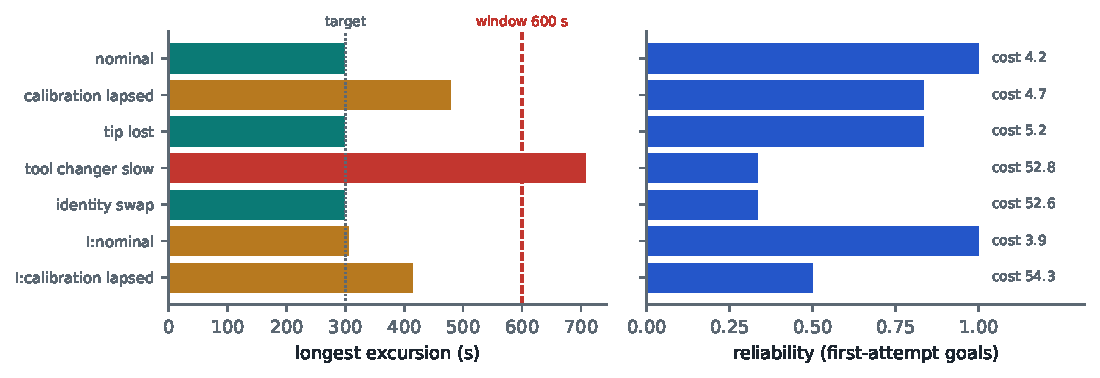
\includegraphics[width=\linewidth]{figures/kpi.pdf}
\caption{KPIs measured from the recorded trails: longest excursion outside the incubator and reliability; cost in the label.}\label{fig:kpi}
\end{figure}

\begin{table}[tbp]\centering\small
\caption{KPIs per recorded run, in the order of the lexicographic ranking.}\label{tab:kpiruns}
\begin{tabularx}{\linewidth}{Xlrrrrr}\toprule
\textbf{Run} & \textbf{End} & \textbf{Safety} & \textbf{Reliability} & \textbf{Auditability} & \textbf{Max excursion (s)} & \textbf{Cost} \\\midrule
nominal & executed & 0 & 1.000 & 1.00 & 298.9 & 4.22 \\
calibration lapsed & executed & 0 & 0.833 & 1.00 & 478.7 & 4.69 \\
tip lost & executed & 0 & 0.833 & 1.00 & 298.9 & 5.24 \\
tool changer slow & escalated & 1 & 0.333 & 1.00 & 708.3 & 52.75 \\
identity swap & escalated & 0 & 0.333 & 1.00 & 298.9 & 52.61 \\
isaac nominal & executed & 0 & 1.000 & 1.00 & 305.7 & 3.89 \\
isaac calibration lapsed & escalated & 0 & 0.500 & 1.00 & 414.6 & 54.28 \\\bottomrule
\end{tabularx}
\end{table}

\section{The culture-level plan}\label{sec:culture}

The culture plan states the experiment over the cultures only. It names the question, the entities (three cultures by role, two substances, a belief over the three models), the goal, what is given, what must never happen (the control is never exposed; no contamination) and what must hold throughout (the cultures' environment). Its steps are what is done to the cultures and what becomes known: challenge, grow, rescue, observe, interpret and analyse. Each step has a physical and a knowledge effect.

\begin{listing}[tbp]
\begin{Verbatim}[fontsize=\footnotesize,breaklines,frame=lines,framesep=2mm]
(the experiment ?E
  (question (which (a recovery-model (in (M1_graded M2_threshold M3_protective)))
                   (explains (the rescue-efficacy (after (a delay (of 48 h)))))))
  (entities
    (the culture ?cr (role rescued))
    (the culture ?cc (role comparator))
    (the culture ?ck (role control))
    (some substance ?ch (type challenge))
    (some substance ?rs (type rescue))
    (the belief ?B (over (M1_graded M2_threshold M3_protective)) (prior uniform)))
  ;; the design guarantees the gain in expectation (e2m); what one execution yields is measured, not promised
  (goal (the belief ?B (expected-information-gain (>= 0.5 bit))))
  (given
    (the culture ?cr (state baseline))
    (the culture ?cc (state baseline))
    (the culture ?ck (state baseline))
    (the belief ?B (entropy 1.585 bit))
    (the experiment ?E (culture-time 0 h)))
  (prevents
    (an exposure (of ?ck) (to (some substance)))           ; the control stays untreated
    (an event (type contamination) (of (a culture))))
  (maintains
    (the culture ?cr (environment culture-standard))
    (the culture ?cc (environment culture-standard))
    (the culture ?ck (environment culture-standard)))
  (steps
\end{Verbatim}
\caption{Head of the culture plan (\texttt{registry/lab/culture\_\allowbreak{}plan.ldl}).}\label{lst:cplan}
\end{listing}

\begin{listing}[tbp]
\begin{Verbatim}[fontsize=\footnotesize,breaklines,frame=lines,framesep=2mm]
(an action ?c3
    (type rescuing)
    (culture ?cr)
    (substance ?rs)
    (dose 0.70 au)
    (at (culture-time 48 h))
    (requires (the experiment ?E (culture-time 48 h)))
    (physical (the culture ?cr (exposed-to ?rs 0.70 au))
              (the culture ?cr (recovery possible)))
    (knowledge (a record (of ?c3) (states ?cr ?rs 0.70 au 48 h))))
\end{Verbatim}
\caption{A culture-level action: the rescue.}\label{lst:culture}
\end{listing}

\begin{table}[tbp]\centering\footnotesize
\caption{Steps of the culture plan with their physical and knowledge effects.}\label{tab:culture_steps}
\begin{tabularx}{\linewidth}{llXX}\toprule
\textbf{Step} & \textbf{Type} & \textbf{Physical effect} & \textbf{Knowledge effect} \\\midrule
?c1 & challenging & \texttt{(the culture ?cr (exposed-\allowbreak{}to ?ch 0.85 au))}; \texttt{(the culture ?cr (injury rising))} & \texttt{(a record (of ?c1) (states ?cr ?ch 0.85 au 0 h))} \\
?c2 & challenging & \texttt{(the culture ?cc (exposed-\allowbreak{}to ?ch 0.85 au))}; \texttt{(the culture ?cc (injury rising))} & \texttt{(a record (of ?c2) (states ?cc ?ch 0.85 au 0 h))} \\
?g1 & growing & \texttt{(the experiment ?E (culture-\allowbreak{}time 48 h))}; \texttt{(the culture ?cr (injury-\allowbreak{}burden accumulated))} & \texttt{(a record (of ?g1) (environment-\allowbreak{}history culture-\allowbreak{}standard))} \\
?c3 & rescuing & \texttt{(the culture ?cr (exposed-\allowbreak{}to ?rs 0.70 au))}; \texttt{(the culture ?cr (recovery possible))} & \texttt{(a record (of ?c3) (states ?cr ?rs 0.70 au 48 h))} \\
?g2 & growing & \texttt{(the experiment ?E (culture-\allowbreak{}time 72 h))}; \texttt{(the culture ?cr (viability settled))} & \texttt{(a record (of ?g2) (environment-\allowbreak{}history culture-\allowbreak{}standard))} \\
?o1 & observing & \texttt{(the culture ?cr (light-\allowbreak{}dose increased))} & \texttt{(an image ?y1 (of ?cr) (culture-\allowbreak{}time 72 h) (raw true))} \\
?o2 & observing & \texttt{(the culture ?cc (light-\allowbreak{}dose increased))} & \texttt{(an image ?y2 (of ?cc) (culture-\allowbreak{}time 72 h) (raw true))} \\
?o3 & observing & \texttt{(the culture ?ck (light-\allowbreak{}dose increased))} & \texttt{(an image ?y3 (of ?ck) (culture-\allowbreak{}time 72 h) (raw true))} \\
?i1 & interpreting & – & \texttt{(an estimate (of ?cr) (organoid-\allowbreak{}radius) (sigma 2.5 um))} \\
?i2 & interpreting & – & \texttt{(an estimate (of ?cc) (organoid-\allowbreak{}radius) (sigma 2.5 um))} \\
?i3 & interpreting & – & \texttt{(an estimate (of ?ck) (organoid-\allowbreak{}radius) (sigma 2.5 um))} \\
?a1 & analysing & – & \texttt{(the belief ?B (posterior updated))}; \texttt{(the belief ?B (information-\allowbreak{}gain measured))} \\\bottomrule
\end{tabularx}
\end{table}

\subsection{Derived order}\label{sec:corder}

The order is derived from 13 causal links, 7 physical and 6 knowledge links (Table~\ref{tab:links}); Fig.~\ref{fig:poset} shows the partial order. One link needs an establishable requirement: interpretation needs a known image scale. It first required "a calibration of the pixel size", which the independence check rejected because calibration is a device function (Section~\ref{sec:indep}).

\begin{figure}[tbp]\centering
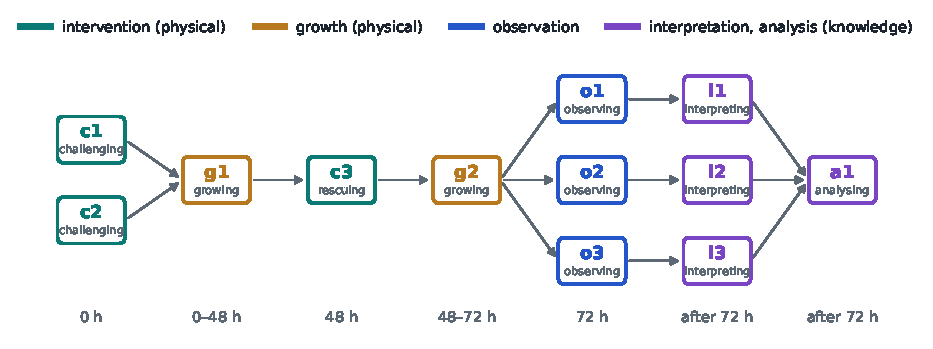
\includegraphics[width=\linewidth]{figures/poset.pdf}
\caption{The culture plan as a partial order (Hasse layers). Colour shows the kind of step.}\label{fig:poset}
\end{figure}

\begin{table}[tbp]\centering\small
\caption{Causal links of the culture plan.}\label{tab:links}
\begin{tabularx}{\linewidth}{lllX}\toprule
\textbf{From} & \textbf{To} & \textbf{Kind} & \textbf{Condition} \\\midrule
?c1 & ?g1 & physical & \texttt{(the culture ?cr (exposed-\allowbreak{}to ?ch))} \\
?c2 & ?g1 & physical & \texttt{(the culture ?cc (exposed-\allowbreak{}to ?ch))} \\
?g1 & ?c3 & physical & \texttt{(the experiment ?E (culture-\allowbreak{}time 48 h))} \\
?c3 & ?g2 & physical & \texttt{(the culture ?cr (exposed-\allowbreak{}to ?rs))} \\
?g2 & ?o1 & physical & \texttt{(the experiment ?E (culture-\allowbreak{}time 72 h))} \\
?g2 & ?o2 & physical & \texttt{(the experiment ?E (culture-\allowbreak{}time 72 h))} \\
?g2 & ?o3 & physical & \texttt{(the experiment ?E (culture-\allowbreak{}time 72 h))} \\
?o1 & ?i1 & knowledge & \texttt{(an image (of ?cr) (raw true))} \\
?o2 & ?i2 & knowledge & \texttt{(an image (of ?cc) (raw true))} \\
?o3 & ?i3 & knowledge & \texttt{(an image (of ?ck) (raw true))} \\
?i1 & ?a1 & knowledge & \texttt{(an estimate (of ?cr) (organoid-\allowbreak{}radius))} \\
?i2 & ?a1 & knowledge & \texttt{(an estimate (of ?cc) (organoid-\allowbreak{}radius))} \\
?i3 & ?a1 & knowledge & \texttt{(an estimate (of ?ck) (organoid-\allowbreak{}radius))} \\\bottomrule
\end{tabularx}
\end{table}

\subsection{Execution on the surrogate and what became known}\label{sec:knowledge}

Run on Cell 01's surrogate, the rescued culture recovers partly and the comparator does not (Fig.~\ref{fig:culture}). The observed effect of 14.8 µm lies between the predictions of M1 and of M2/M3, so the belief moves towards M1 but gains only 0.357 bit, against 0.5 bit required and 0.5439 bit expected. The design meets the requirement only in expectation; the goal therefore says \texttt{expected-\allowbreak{}information-\allowbreak{}gain}. A priming design that separates M2 from M3 is on the roadmap.

\begin{figure}[tbp]\centering
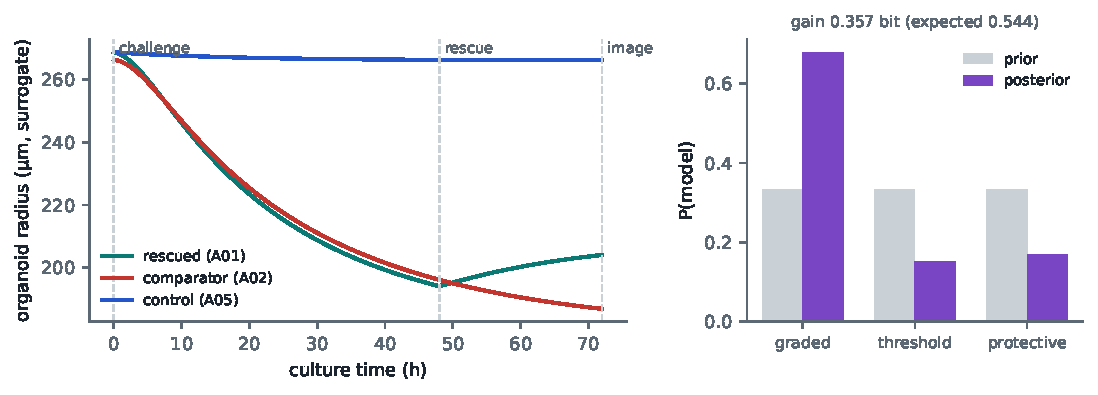
\includegraphics[width=\linewidth]{figures/culture.pdf}
\caption{Surrogate organoid radii of the three cultures over culture time (left) and the belief over the recovery models before and after the experiment (right). ILLUSTRATIVE.}\label{fig:culture}
\end{figure}

\begin{table}[tbp]\centering\small
\caption{What the experiment made known (surrogate, ILLUSTRATIVE).}\label{tab:knowledge}
\begin{tabularx}{\linewidth}{Xl}\toprule
\textbf{Quantity} & \textbf{Value} \\\midrule
observed radius A01 / A02 / A05 (µm) & 201.6 / 186.8 / 267.6 \\
measurement noise σ (µm) & 2.49 \\
observed rescue effect (µm) & 14.76 \\
predicted effect M1 / M2 / M3 (µm) & 8.5 ± 11.4 / 25.0 ± 6.3 / 25.4 ± 6.5 \\
posterior M1 / M2 / M3 & 0.678 / 0.152 / 0.170 \\
entropy before / after (bit) & 1.585 / 1.228 \\
information gained (bit) & 0.357 \\
expected gain of the design / required (bit) & 0.5439 / 0.5 \\\bottomrule
\end{tabularx}
\end{table}

\subsection{Mapping to the laboratory}\label{sec:mapping}

The cultures map to wells A01, A02 and A05 of plate P17; the eight physical culture actions map to lab action designators and, through their instrument roles, to L12, L10 and L17. The four computations (interpretation and analysis) map to the twin's image analysis and posterior computation. The lab order is exactly the projection of the culture order.

\begin{table}[tbp]\centering\small
\caption{Refinement of the culture actions to lab actions, processes and devices.}\label{tab:refine}
\begin{tabularx}{\linewidth}{lllX}\toprule
\textbf{Culture action} & \textbf{Lab action} & \textbf{Process} & \textbf{Realized by} \\\midrule
?c1 challenging & ?x1 intervening & substance-transfer & L12 \\
?c2 challenging & ?x2 intervening & substance-transfer & L12 \\
?g1 growing & ?w1 incubating & incubation & L10 \\
?c3 rescuing & ?x3 intervening & substance-transfer & L12 \\
?g2 growing & ?w2 incubating & incubation & L10 \\
?o1 observing & ?m1 measuring & imaging & L17 \\
?o2 observing & ?m2 measuring & imaging & L17 \\
?o3 observing & ?m3 measuring & imaging & L17 \\
?i1 interpreting &  computation &  & culture SDT image analysis (twin/culture/optics.analyse): radius from the calibrated pixel size \\
?i2 interpreting &  computation &  & culture SDT image analysis (twin/culture/optics.analyse): radius from the calibrated pixel size \\
?i3 interpreting &  computation &  & culture SDT image analysis (twin/culture/optics.analyse): radius from the calibrated pixel size \\
?a1 analysing &  computation &  & posterior over M1-M3 (twin/culture/eig.posterior\_\allowbreak{}over\_\allowbreak{}models) on the rescued - comparator radius \\\bottomrule
\end{tabularx}
\end{table}

\begin{table}[tbp]\centering\small
\caption{Instantiation of the abstract entities in Cell 01.}\label{tab:instantiation}
\begin{tabularx}{\linewidth}{llX}\toprule
\textbf{Abstract entity} & \textbf{Role} & \textbf{Particular in Cell 01} \\\midrule
\texttt{?cr} & rescued & the organoid in P17:A01 \\
\texttt{?cc} & comparator & the organoid in P17:A02 \\
\texttt{?ck} & control & the organoid in P17:A05 \\
\texttt{?ch} & challenge & reagent abstract\_\allowbreak{}challenge\_\allowbreak{}reagent (barcode RGT-0001, lot SIM-LOT-A) at l12\_\allowbreak{}liquidhandler\_\allowbreak{}reagent\_\allowbreak{}rack\_\allowbreak{}frames\_\allowbreak{}rack\_\allowbreak{}1\_\allowbreak{}pos\_\allowbreak{}1 \\
\texttt{?rs} & rescue & reagent abstract\_\allowbreak{}rescue\_\allowbreak{}reagent (barcode RGT-0002, lot SIM-LOT-B) at l12\_\allowbreak{}liquidhandler\_\allowbreak{}reagent\_\allowbreak{}rack\_\allowbreak{}frames\_\allowbreak{}rack\_\allowbreak{}1\_\allowbreak{}pos\_\allowbreak{}2 \\
\texttt{(the plate ?p)} & carrier & Plate\_\allowbreak{}P17 in L10 cassette slot 2 \\\bottomrule
\end{tabularx}
\end{table}

\textbf{Feasibility.} For each session the assistant checks every transport leg (both seats served by the robot, reach from the layout, seats typed in the SDT), the tool coupling, the machine tending of L10, L12 and L17, and the trip time against the window. All checks pass, with evidence from facts and from the Isaac run. They are conditional on two assumed device preconditions (L12 calibrated, L17 healthy), and inventory (tips, reagent stock) is not modelled.

\begin{table}[tbp]\centering\small
\caption{Feasibility checks per session.}\label{tab:feas}
\begin{tabularx}{\linewidth}{lllXrl}\toprule
\textbf{Session} & \textbf{Culture time} & \textbf{Device} & \textbf{Transport legs} & \textbf{Checks} & \textbf{All pass} \\\midrule
s0 & 0 h & L12 & R01 L10→HANDOVERNEST; R02 HANDOVERNEST→L12; R02 L12→HANDOVERNEST; R01 HANDOVERNEST→L10 & 8 & yes \\
s1 & 48 h & L12 & R01 L10→HANDOVERNEST; R02 HANDOVERNEST→L12; R02 L12→HANDOVERNEST; R01 HANDOVERNEST→L10 & 8 & yes \\
s2 & 72 h & L17 & R01 L10→HANDOVERNEST; R02 HANDOVERNEST→L17; R02 L17→HANDOVERNEST; R01 HANDOVERNEST→L10 & 8 & yes \\\bottomrule
\end{tabularx}
\end{table}

\section{Execution}\label{sec:exec}

The executive turns one linear extension of the lab plan, grouped by culture time into sessions, into a plan tree. The generalized plan of each category builds its sub-plan at perform time, querying the knowledge base; the leaves are motions and device commands. Before anything moves, the whole experiment is projected from the assistant's belief (F6, F12): every designator must be groundable, the understanding gate must accept every card, and the window policies predict instead of abort (F8). At each session start, observations of shared cell state go stale and are re-established (F2). If a session fails after the plate left the incubator, an unwind-protect returns it before the failure propagates, unless it was quarantined (F10).

The executive is also emitted as a CRAM/RPL structured reactive controller (409 lines of Lisp): one \texttt{def-\allowbreak{}action-\allowbreak{}plan} per lab action type, with the contract's requires as checks, the scoped prevents as monitors, and the handlers as failure handling. Listing~\ref{lst:cram} shows the plan for \texttt{intervening}.

\begin{listing}[tbp]
\begin{Verbatim}[fontsize=\footnotesize,breaklines,frame=lines,framesep=2mm]
(def-action-plan intervening ((into ?w) (substance ?s) (dose ?q) (at ?t))
  "Goal: (the well ?w (received ?s ?q)). Performed in: x1, x2, x3."
  (let* ((?self (current-action-designator))
         (?p (plate-of ?w))
         (?instrument (an instrument
                          (slot (a plate-slot (accepts ?p)))
                          (process (a process
                                       (type substance-transfer)
                                       (into ?w)
                                       (of ?s)
                                       (amount ?q))))))
    (with-retry-counters ((wrong-reagent-repairs 1) (tip-missing-or-dropped-repairs 1))
      (with-failure-handling
          ((dose-not-delivered (f)
             (case (failure-cause f)
               ;; perform again; guarantees goal-or-safe-state: holds
               (wrong_reagent (do-retry wrong-reagent-repairs
                                (achieve (some substance ?s (identity verified)))
                                (retry)))
               ;; perform again; guarantees goal-or-safe-state: holds
               (tip_missing_or_dropped (do-retry tip-missing-or-dropped-repairs (retry))))))
        (seq
          (ensure (the plate ?p (identity verified))
                  :grade (freshness fresh source observed)
                  :consequential t)
          (ensure (some substance ?s (identity verified))
                  :grade (freshness fresh source observed)
                  :consequential t)
          (ensure (the plate ?p (contamination none))
                  :grade (freshness fresh source inferred)
                  :consequential t)
          ;; supplied by a predecessor in the partial order
          (wait-for (holds (the plate ?p (culture-time ?t))))
          (with-policy (par
                         (prevent (holds (an event (type contamination-introduced) (of ?p)))
                                  contamination-suspected)
                         (scope ((holds (a portion ?u (of ?s) (drawn-for ?self)))
                                 (holds (the portion ?u (delivered true))))
                           (prevent (holds (a transfer (of ?u) (into (a well (of ?p) (not ?w)))))
                                    prevents-violated)))
            (perform (an action (type tending) (instrument ?instrument) (object ?p))))
          (check-goal (the well ?w (received ?s ?q)) dose-not-delivered))))))
\end{Verbatim}
\caption{The generated CRAM/RPL plan for the lab action type \texttt{intervening}.}\label{lst:cram}
\end{listing}

\subsection{Cross-check with the planner}\label{sec:crosscheck}

Expanding the nominal plan into designators reproduces the clingo plan's leaf steps term for term (153 leaves, same primitive, agent and pose, in the same order), and the durations match the planner's exactly (298.9, 263.3, 256.4 s). Two independent derivations from the same facts agree. Since the symbolic backend takes durations from the planner's facts, this shows consistency, not independent physics; the Isaac runs supply the latter.

\begin{figure}[tbp]\centering
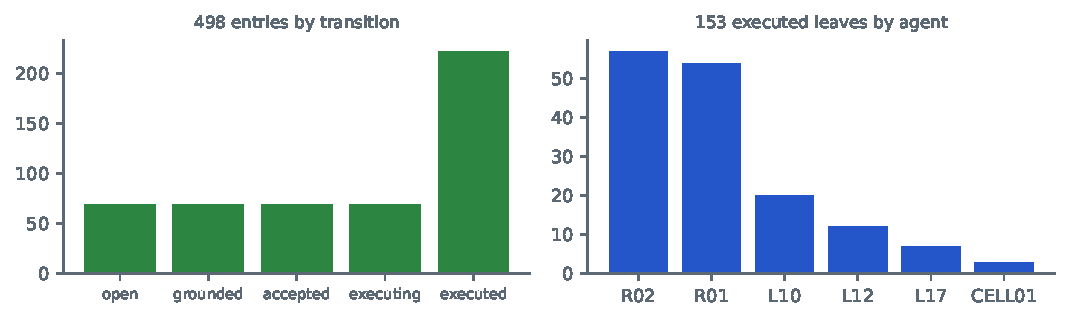
\includegraphics[width=\linewidth]{figures/trail.pdf}
\caption{The nominal audit trail: entries by lifecycle transition and executed leaves by agent.}\label{fig:trail}
\end{figure}

\subsection{Scenarios}\label{sec:scenarios}

Twelve symbolic scenarios exercise the kernel with the \emph{same plan code}; only knowledge and world change (Table~\ref{tab:scen_cat}). Expectations, including the two-column verdict and the disposition, were written before the runs. They cover device exchange, step substitution by knowledge and by repair, workflow change, safety and identity, and knowledge gaps.

\begin{table}[tbp]\centering\footnotesize
\caption{Scenario catalogue: what is injected and how each run ends.}\label{tab:scen_cat}
\begin{tabularx}{\linewidth}{lXX}\toprule
\textbf{Scenario} & \textbf{Fault or change injected} & \textbf{Outcome} \\\midrule
nominal & the derived 0.5-bit experiment, fault-free & executed \\
calibration lapsed & the KB believes L17 calibrated but it lapsed; detected at imaging, repaired by QC and re-imaging & executed \\
card incomplete & the dose category card lacks its evidence obligations; the understanding gate refuses the dose & abstained: refused: refused by projection\_\allowbreak{}succeeds \\
contamination & contamination is suspected; challenge and rescue are refused & abstained: refused: refused by projection\_\allowbreak{}succeeds, contamination\_\allowbreak{}free \\
control dropped & the workflow is changed to drop the control well; the experiment is refused before any motion & abstained: refused: refused by projection\_\allowbreak{}succeeds, challenge\_\allowbreak{}requires\_\allowbreak{}controls \\
identity swap & L10 holds P18 instead of P17 at the rescue session; quarantine P18, escalate & escalated: escalated: l10 read P18, expected P17 (after quarantine P18 (Cell 01 routing H4\_\allowbreak{}quarantine\_\allowbreak{}if\_\allowbreak{}identity\_\allowbreak{}unresolved); P17 location… \\
imager incapable & L17 replaced by a device without well imaging; the measurement session cannot be grounded & abstained: refused: refused by projection\_\allowbreak{}succeeds \\
imager swapped & L17 replaced by a capability-matched imager without a validated binding for the readout (device exchange) & executed \\
rescue unbound & the rescue reagent is not bound to a rack position; the rescue dose cannot be grounded & abstained: refused: refused by projection\_\allowbreak{}succeeds \\
tip lost & the tip falls off after the pick at the rescue dose; detected before aspiration, tip replaced & executed \\
tool changer slow & the tool changer takes 600 s at the rescue session; window exceeded, safe return & escalated: session\_\allowbreak{}failed: policy window: 645.3 s outside the incubator (window 600.0 s) (after safe return of the plate to its controlled … \\
uncalibrated known & the KB does not assert calibrated(l17); a QC calibration is planned before imaging (step insertion by knowledge) & executed \\
isaac nominal & the derived 0.5-bit experiment on the Cell 01 twin & executed \\
isaac calibration lapsed & L17's calibration is invalidated just before the first image of s2; set aside, recalibrate at L21, re-plan & escalated: session\_\allowbreak{}failed: A02 out of focus; retained (after safe return of the plate to its controlled environment (focus\_\allowbreak{}invalid in measu… \\
isaac identity swap & the experiment is about P18 (L10 inventory slot 5) but the plate in slot 5 is P23 (twin initial state); L10's barcode read catches it, P23 is quarantined in H4, escalation & escalated: escalated: l10 read P23, expected P18 (after quarantine P23 (Cell 01 routing H4\_\allowbreak{}quarantine\_\allowbreak{}if\_\allowbreak{}identity\_\allowbreak{}unresolved); P18 location… \\\bottomrule
\end{tabularx}
\end{table}

\begin{table}[tbp]\centering\footnotesize
\caption{Outcome per scenario: end state, realization (R) and validity (V), repairs, trail size, and whether it ended as specified.}\label{tab:scenarios}
\begin{tabularx}{\linewidth}{lllllrl}\toprule
\textbf{Scenario} & \textbf{Backend} & \textbf{End} & \textbf{R | V} & \textbf{Repairs} & \textbf{Entries} & \textbf{As specified} \\\midrule
nominal & symbolic & executed & ok | ok & – & 498 & yes \\
calibration lapsed & symbolic & executed & ok | ok & image & 569 & yes \\
card incomplete & symbolic & abstained & – | – & – & 3 & yes \\
contamination & symbolic & abstained & – | – & – & 3 & yes \\
control dropped & symbolic & abstained & – | – & – & 3 & yes \\
identity swap & symbolic & escalated & – | – & retrieve & 224 & yes \\
imager incapable & symbolic & abstained & – | – & – & 3 & yes \\
imager swapped & symbolic & executed & ok | – & – & 498 & yes \\
rescue unbound & symbolic & abstained & – | – & – & 3 & yes \\
tip lost & symbolic & executed & ok | ok & dose & 501 & yes \\
tool changer slow & symbolic & escalated & – | – & run\_\allowbreak{}session & 266 & yes \\
uncalibrated known & symbolic & executed & ok | ok & – & 504 & yes \\
nominal & Isaac Sim & executed & ok | ok & – & 498 & yes \\
calibration lapsed & Isaac Sim & escalated & – | – & run\_\allowbreak{}session, image, image & 562 & NO \\
identity swap & Isaac Sim & escalated & – | – & retrieve & 56 & yes \\\bottomrule
\end{tabularx}
\end{table}

\begin{itemize}
  \item \textbf{Device exchange.} \texttt{imager\_\allowbreak{}swapped} executes unchanged and ends NR3: physically realised, invalid evidence, nothing committed. \texttt{imager\_\allowbreak{}incapable} is refused before the first intervention, naming the missing capability.
  \item \textbf{Step substitution.} \texttt{uncalibrated\_\allowbreak{}known} inserts a QC calibration as a preparation step. \texttt{calibration\_\allowbreak{}lapsed} detects the lapse at imaging, sets the plate aside at a passive station, recalibrates and re-plans the measurement. \texttt{tip\_\allowbreak{}lost} replaces the tip before aspiration.
  \item \textbf{Workflow change.} \texttt{control\_\allowbreak{}dropped} is refused by \texttt{challenge\_\allowbreak{}requires\_\allowbreak{}controls} before anything moves.
  \item \textbf{Safety and identity.} \texttt{identity\_\allowbreak{}swap} quarantines the wrong plate, escalates, and records that it does not know where P17 is. \texttt{tool\_\allowbreak{}changer\_\allowbreak{}slow} exceeds the window and returns the plate before reporting failure.
  \item \textbf{Knowledge gaps.} \texttt{rescue\_\allowbreak{}unbound}, \texttt{contamination} and \texttt{card\_\allowbreak{}incomplete} are refused before any motion.
\end{itemize}

\subsection{Isaac Sim execution}\label{sec:isaac}

The Isaac backend runs the same plan code, knowledge, audit, critic and competency questions; only leaf execution changes. The twin's skills are coarser than the leaves (F13): a robot pick is approach, insert, grasp and lift; L12's \texttt{dose\_\allowbreak{}well} is tip pick, aspirate, dispense and tip eject. A group of leaves is executed at its first leaf, and the following leaves report the phases of that execution; every leaf entry records what realised it. Durations are physics time; culture waits advance a separate clock.

\begin{figure}[tbp]\centering
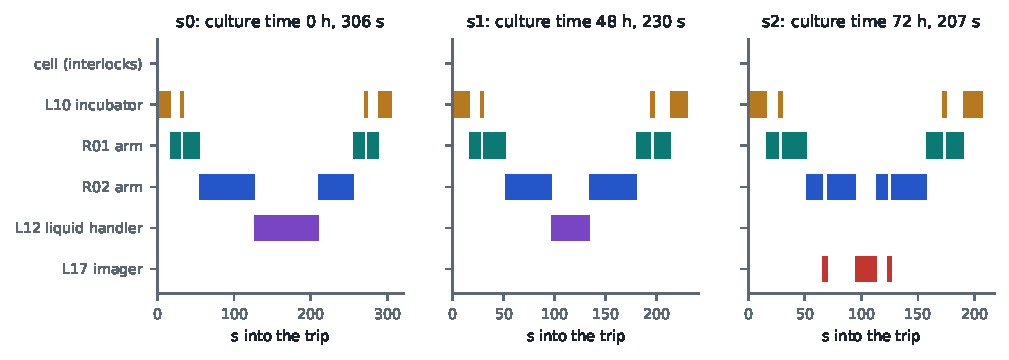
\includegraphics[width=\linewidth]{figures/gantt.pdf}
\caption{The nominal run in Isaac Sim: leaves per agent over each session.}\label{fig:gantt}
\end{figure}

The twin's session durations deviate from the planner's by +2.3 \%, -12.6 \%, -19.1 \% and stay within the window. \texttt{isaac\_\allowbreak{}identity\_\allowbreak{}swap} ends as specified: L10 read the wrong barcode, the plate was quarantined at H4 and the run escalated.

**Finding F17: \texttt{isaac\_\allowbreak{}calibration\_\allowbreak{}lapsed} does not end as specified.** The calibration repair worked: L17 refused, the plate was set aside, L21 recalibrated and the measurement was re-planned; A01 was then imaged validly. A02 then failed the focus floor twice (scores 0.035 and 0.030, floor 0.04); the session returned the plate and escalated, so control A05 was never imaged. After the reload, the A01 field is shifted by about 93 µm against the nominal run with the same commanded stage position and seat sensors at zero gap; two A02 images of the same load differ by about 35 µm. The plate seems to move in the nest, which the seat sensors do not see. The kernel's repair \texttt{focus\_\allowbreak{}invalid → autofocus, retry} cannot change the outcome, because L17 autofocuses before every image; the process model prescribes a re-seat, and the LDL checker catches the refocus-only handler (N9). The disposition was correct for what happened; the expected outcome was not reached, and the expectation was not changed.

\section{Audit trail, critic and competency questions}\label{sec:audit}

Every lifecycle transition of every designator writes one commitment record: sequence number, simulated time, designator and parent, kind and category, transition, agent and software versions, the HADL term, bindings, resolution grounds, constraint verdicts, monitor results and evidence references, each with its own SHA-256. Each entry carries the hash of its predecessor and its own hash over the canonical JSON, forming a chain~\citep{haber1991}. A verifier recomputes the chain; editing any value breaks it at that entry. Listing~\ref{lst:audit} shows a dispense entry.

\begin{listing}[tbp]
\begin{Verbatim}[fontsize=\footnotesize,breaklines,frame=lines,framesep=2mm]
{
  "seq": 86,
  "t_sim": 156.1,
  "designator": "d0039-dispense",
  "parent": "d0036-dose",
  "kind": "command",
  "category": "dispense",
  "transition": "executed",
  "agent": "l12",
  "software": {"kernel": "rsa-kernel/0.1", "kb": "facts_g050+nominal", "registry": "5d901b7f8087...
  "term": ["cmd", "l12", ["dispense", "https___aicor_example_okf_sdt_lab1_world_experimentalworl...
  "monitors": [{"name": "well_binding", "passed": true, "observation": "P17/A01"}, {"name": "dis...
  "constraints": [{"id": "l12_airspace_clear", "column": "realization", "verdict": "ENFORCED", "...
  "evidence": [  // 10 items, each with its own sha256
    {"kind": "plate", "value": "P17", "sha256": "6f418d76902ea3669355d6f0f3abf4387fe78c83d8b...,
    {"kind": "well", "value": "A01", "sha256": "3b1d4717064134258d9fc1cdb2a8055c242348548558...,
    {"kind": "reagent", "value": "challenge", "sha256": "d0303e386ced87e527d925fae2b47bbbf40...,
    ...],
  "prev": "32dddeae06c3eed2acaa64bf9e9f446a834a8539ff4e35f1ec28bf0ded3ce3b9",
  "hash": "e890f45744b3ada383becbcd869882c65acd04239017d16b015f077ee6d9c739",
}
\end{Verbatim}
\caption{An audit entry of the nominal trail (a dispense), abbreviated.}\label{lst:audit}
\end{listing}

\textbf{Critic.} The critic judges each episode from the trail alone, in two columns. Realization: the run ended executed and no runtime constraint was violated. Validity: V1–V7 (identity continuity, calibration at measurement, validated binding, controls measured, dose delivered, sample integrity, design realised). The result may update the culture belief only if both hold (D009).

\subsection{Competency questions}\label{sec:cq}

27 competency questions in 13 families ask what the assistant is doing, why, how, under which constraints, with which capability, what would happen if, with what evidence, what went wrong, which norms are covered, whether the result is valid, what it does not know, what kind of action something is, and what a device exchange would change. They are answered from the trail, the knowledge base and dry runs, with grounds. Expected answers were written by hand for selected scenarios before the runs: 52 checks, 52 correct and all grounded.

\begin{table}[tbp]\centering\small
\caption{Competency-question checks by family.}\label{tab:cqfam}
\begin{tabularx}{\linewidth}{Xrr}\toprule
\textbf{Family} & \textbf{Checks} & \textbf{Correct} \\\midrule
what & 3 & 3 \\
why & 4 & 4 \\
how & 2 & 2 \\
constraints & 3 & 3 \\
capability & 4 & 4 \\
what-if & 3 & 3 \\
evidence & 4 & 4 \\
retrospective & 13 & 13 \\
normative & 4 & 4 \\
verdict & 8 & 8 \\
epistemic & 2 & 2 \\
taxonomy & 1 & 1 \\
modularity & 1 & 1 \\\bottomrule
\end{tabularx}
\end{table}

\begin{listing}[tbp]
\begin{Verbatim}[fontsize=\footnotesize,breaklines,frame=lines,framesep=2mm]
{
 "id": "CQ-03",
 "scenario": "nominal",
 "question": "Why was this device chosen for dosing, and which alternatives were rejected?",
 "answer": {
  "device": "l12",
  "grounds": [
   "automated(l12)",
   "has_function(l12,dispensing)",
   "component:L12_LiquidHandler.capabilities in dose_well"
  ],
  "rejected": []
 },
 "grounds": [
  "trail#81:dose/grounded",
  "automated(l12)",
  "has_function(l12,dispensing)",
  "component:L12_LiquidHandler.capabilities in dose_well"
 ]
}
\end{Verbatim}
\caption{An answer with grounds: why L12 was chosen for dosing and which devices were rejected (CQ-03, nominal).}\label{lst:cq}
\end{listing}

\subsection{The kernel in the ontology}\label{sec:okf}

The kernel's categories and the trail are exported to an OKF module. Each category is a class defined by its level and kernel name, so trail individuals are classified by the reasoner; effect classes and facets are disjoint superclasses aligned with the e2m designator classes. HermiT finds no unsatisfiable class after F14; Konclude realises 6244 individuals, and all 222 designators and 498 audit entries of the nominal trail are classified with none left over. 18 TBox competency questions and 6 negative controls pass.

\section{Motion level}\label{sec:motion}

Every motion leaf of the executed plan is refined into a Giskard motion designator: 111 leaves become 111 designators over 12 legs, 6 of them distinct. Each designator has reference frames (robot root and tip, and a goal pose in a seat frame of the composed scene), motion constraints (Cartesian goal or straight line, speed limits, plate kept level, collision avoidance, allowed contacts), an ending monitor and cancel conditions, and the objective of giskardpy's QP-based model-predictive controller. The output is a Lisp description and a giskardpy module of 1958 lines whose API use was checked against a CRAM checkout.

\begin{table}[tbp]\centering\small
\caption{Distinct transport legs and their motion sequences.}\label{tab:legs}
\begin{tabularx}{\linewidth}{llrX}\toprule
\textbf{Robot} & \textbf{Leg} & \textbf{Motions} & \textbf{Sequence} \\\midrule
R01 & L10 → HANDOVERNEST & 9 & approaching → inserting → grasping → lifting → transiting → aligning → placing → releasing → retracting \\
R02 & HANDOVERNEST → L12 & 10 & coupling → approaching → inserting → grasping → lifting → transiting → aligning → placing → releasing → retracting \\
R02 & L12 → HANDOVERNEST & 9 & approaching → inserting → grasping → lifting → transiting → aligning → placing → releasing → retracting \\
R01 & HANDOVERNEST → L10 & 9 & approaching → inserting → grasping → lifting → transiting → aligning → placing → releasing → retracting \\
R02 & HANDOVERNEST → L17 & 10 & coupling → approaching → inserting → grasping → lifting → transiting → aligning → placing → releasing → retracting \\
R02 & L17 → HANDOVERNEST & 9 & approaching → inserting → grasping → lifting → transiting → aligning → placing → releasing → retracting \\\bottomrule
\end{tabularx}
\end{table}

\begin{table}[tbp]\centering\small
\caption{Controller parameters and motion bounds.}\label{tab:giskard}
\begin{tabularx}{\linewidth}{p{2.6cm}XX}\toprule
\textbf{Parameter} & \textbf{Value} & \textbf{Meaning} \\\midrule
control frequency & 50 Hz (dt 0.02 s) & QP-based MPC rate \\
prediction horizon & 7 & steps; highest derivative jerk; solver PIQP \\
weights & level 2500, speed 2500, collision 50, goal 1, posture 0.1 & level and speed dominate; goal tracking is soft \\
plate tilt & ≤ 2.0° & kept level while held (cancel if violated) \\
transit speed & ≤ 0.25 m/s, 0.6 rad/s & Cartesian limits while carrying \\
pose tolerance & 0.4 mm, 0.2° & end monitor at grasp / release (A3) \\
lock gap & 4 mm & nest capture before release \\
timeout & 1.2 × estimate & the ±20 \% duration bound of z3 theorem V3 \\\bottomrule
\end{tabularx}
\end{table}

\begin{listing}[tbp]
\begin{Verbatim}[fontsize=\footnotesize,breaklines,frame=lines,framesep=2mm]
def inserting(world, robot, seat, z, speed, tol, plate):
    root, tcp = body(world, robot["root"]), body(world, robot["tcp"])
    goal = tool_down(body(world, seat), z)
    done = PoseReached(root_link=root, tip_link=tcp, goal_pose=goal.to_homogeneous_matrix(),
                       position_threshold=tol, orientation_threshold=ORI_TOL)
    aux = [CartesianPoseStraight(root_link=root, tip_link=tcp, goal_pose=goal),
           CartesianPositionVelocityLimit(root_link=root, tip_link=tcp, max_linear_velocity=speed, weight=W_SPEED),
           allow_contact([body(world, j) for j in robot["finger_links"]], [plate])]
    return done, aux


def straight(world, robot, seat, z, speed, plate=None, contact=None):
    """lifting, placing, retracting: straight vertical motion of the TCP at a capped speed."""
    root, tcp = body(world, robot["root"]), body(world, robot["tcp"])
    done = CartesianPositionStraight(root_link=root, tip_link=tcp,
                                     goal_point=Point3(0.0, 0.0, z, reference_frame=body(world, seat)),
                                     reference_velocity=speed, threshold=POSE_TOL)
    aux = [CartesianPositionVelocityLimit(root_link=root, tip_link=tcp, max_linear_velocity=speed, weight=W_SPEED)]
    if plate is not None:
        aux.append(keep_level(world, plate))
    if contact is not None:
        aux.append(allow_contact(*contact))
    return done, aux
\end{Verbatim}
\caption{The generated giskardpy statechart for inserting into a seat.}\label{lst:giskard}
\end{listing}

All 25 goal frames are reachable with the FR3 and the rail-mounted UR5e kinematics within joint-margin and conditioning thresholds (Fig.~\ref{fig:reach}). R01's goals are collision-free; R02's collisions are not checked offline. Compliant insertion is open: giskardpy has no impedance control, and a force monitor needs ROS.

\begin{figure}[tbp]\centering
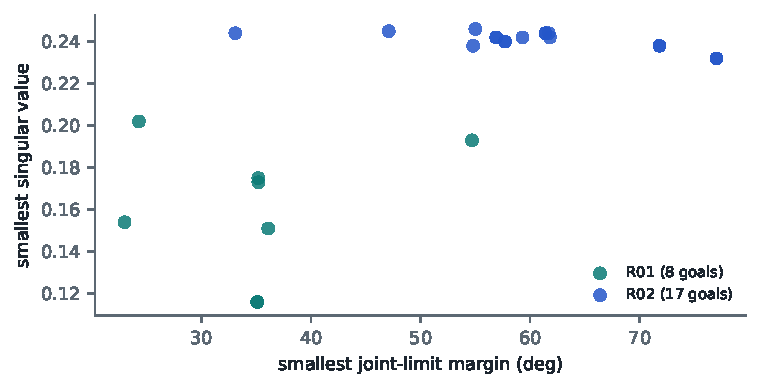
\includegraphics[width=0.72\linewidth]{figures/reach.pdf}
\caption{Reachability of the goal frames: joint-limit margin and smallest singular value of the Jacobian per goal.}\label{fig:reach}
\end{figure}

\section{Refinement proof}\label{sec:proof}

The refinement proof shows that the motion-level plan executes the culture-level plan and satisfies the stated constraints, relative to explicit assumptions about controllers, sensors and devices. It is an assume-guarantee argument in the sense of refinement mappings and contract-based design~\citep{abadi1991,benveniste2018}.

\textbf{Theorem.} Let Π\_\allowbreak{}M be the motion-level plan of the experiment: the 151 grounded steps whose 111 robot motions are refined into Giskard statecharts. Under A1–A6, every execution of Π\_\allowbreak{}M either (i) realizes the culture plan: every physical and knowledge effect in the derived order at the design's culture times, with the control untreated, while every stated constraint holds on the way (interlocks, L12 airspace, identity, environment before store, calibration before imaging, the window, contamination freedom, tool hygiene, plate level, collision distance); or (ii) is stopped by a monitor and ends in a failure handler whose guarantee holds (safe state, contained, or the goal).

\begin{table}[tbp]\centering\small
\caption{Assumptions of the refinement proof.}\label{tab:assumptions}
\begin{tabularx}{\linewidth}{lXl}\toprule
\textbf{} & \textbf{Assumption} & \textbf{Covered by} \\\midrule
A1 & a motion statechart ends only through EndMotion (its end monitor true) or CancelMotion. & library semantics \\
A2 & PoseReached, LocalMinimumReached with the grasp check, VectorsAligned, the collision distance monitors, the simulation clock, the barcode read, the seat sensors and the device monitors observe correctly. & assumed; 2 fault kinds only partly detected \\
A3 & a TCP within 0.4 mm / 0.2 deg of a seat's grasp or release pose has the plate in that seat (the nest guides capture it); within 5 mm of an approach pose it is at that approach pose (free-space waypoint). & ILLUSTRATIVE capture (2 mm) \\
A4 & grasp\_\allowbreak{}confirmed, lifted, seating). & monitored at run time \\
A5 & dose\_\allowbreak{}well delivers within its tolerance when its monitors pass; image\_\allowbreak{}well yields an image when calibration and focus monitors pass; L10 holds the environment profile while the plate is stored. & component contracts, monitored \\
A6 & the goal frames are the ones the scene defines (rsa/motion\_\allowbreak{}frames.py), and each is reachable (checked).  & checked (25/25) \\\bottomrule
\end{tabularx}
\end{table}

\begin{figure}[tbp]\centering
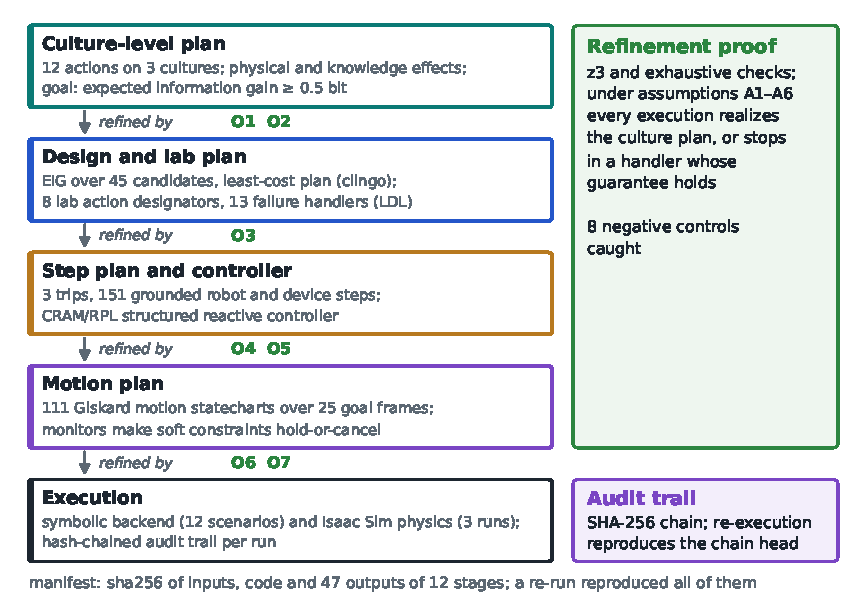
\includegraphics[width=0.9\linewidth]{figures/chain.pdf}
\caption{The proof chain: levels, the obligation discharged between each pair, and the audit.}\label{fig:chain}
\end{figure}

\begin{table}[tbp]\centering\small
\caption{Proof obligations and how they are discharged.}\label{tab:obligations}
\begin{tabularx}{\linewidth}{lXll}\toprule
\textbf{} & \textbf{Obligation} & \textbf{Discharged by} & \textbf{Result} \\\midrule
O1 & culture plan well formed (supported, acyclic) & causal-link analysis & 13 links \\
O2 & step-level events entail every culture effect, the order and the culture prevents & z3 (negation UNSAT) & 14/14 \\
O3 & lab plan: links, threats, instruments, handler guarantees & LDL checker & threats 9/9, guarantees 13/13 \\
O4 & step plan: executability, safety, time, realization, gain, least cost & z3 (V1–V5) & 7/7 theorems \\
O5 & no plate-handling tool touches the culture & z3 & holds \\
O6 & each motion refines its step; end monitor implies the postcondition; soft parts hold-or-cancel & exhaustive check & 111/111 motions \\
O7 & every cancellation reaches a handler with a verified guarantee & exhaustive check & 13 failure types \\\bottomrule
\end{tabularx}
\end{table}

\begin{table}[tbp]\centering\small
\caption{Obligation O2: every culture-level effect is entailed by step-level events (z3).}\label{tab:o2}
\begin{tabularx}{\linewidth}{Xl}\toprule
\textbf{O2 obligation (culture-level effect entailed by step-level events)} & \textbf{Proved} \\\midrule
?c1 challenging ?cr: exposed to challenge 0.85 au at 0 h & yes \\
?c2 challenging ?cc: exposed to challenge 0.85 au at 0 h & yes \\
?g1 growing 0 -> 48 h: cultures in their environment between the trips & yes \\
?c3 rescuing ?cr: exposed to rescue 0.70 au at 48 h & yes \\
?g2 growing 48 -> 72 h: cultures in their environment between the trips & yes \\
?o1 observing ?cr: image at 72 h & yes \\
?o2 observing ?cc: image at 72 h & yes \\
?o3 observing ?ck: image at 72 h & yes \\
?i1 interpreting ?cr: image and known scale & yes \\
?i2 interpreting ?cc: image and known scale & yes \\
?i3 interpreting ?ck: image and known scale & yes \\
?a1 analysing: estimates of the rescued, comparator and control cultures & yes \\
prevents: the control culture is never exposed & yes \\
order: challenges at 0 h < rescue at 48 h < observations at 72 h & yes \\\bottomrule
\end{tabularx}
\end{table}

Motion constraints are hold-or-cancel: a statechart ends only through its end monitor or a cancel, and every cancel (timeout at 1.2 × the estimate, tilt, collision distance) reaches a handler with a verified guarantee (O7). The proof does not cover progress (that a motion terminates), the two partly detected faults, contact physics, or Giskard's execution itself.

\begin{table}[tbp]\centering\small
\caption{Negative controls of the refinement proof.}\label{tab:negative}
\begin{tabularx}{\linewidth}{Xl}\toprule
\textbf{Mutation} & \textbf{Caught} \\\midrule
vessel map swaps rescued and comparator & yes \\
the control well A05 is also dosed & yes \\
the control well is not imaged & yes \\
the plate tool T01 touches the culture & yes \\
one held motion without the tilt cancel & yes \\
one motion's timeout beyond V3's bound (1.5 x) & yes \\
a motion that does not refine its step & yes \\
step level: the validator's own 10 mutated plans & yes \\\bottomrule
\end{tabularx}
\end{table}

\section{Independence of the culture plan}\label{sec:indep}

The culture plan must not depend on the laboratory. Two checks establish this. \textbf{Vocabulary:} no term of six realization vocabularies (robots, devices, lab setup, safety constraints, cleanliness, temperature control), collected from the facts, the component records and the registries, occurs in the culture plan. The check found one leak, a requirement for "a calibration of the pixel size"; it now requires a known image scale. \textbf{Invariance:} in 13 laboratory variants the culture plan, its order and the lab plan are identical; only the realization differs, and some laboratories refuse before anything moves (Table~\ref{tab:labs}).

\begin{table}[tbp]\centering\footnotesize
\caption{The culture plan in 13 laboratory variants. The culture-plan hash is the same in all.}\label{tab:labs}
\begin{tabularx}{\linewidth}{Xlll}\toprule
\textbf{Lab variant} & \textbf{Dimension} & \textbf{Outcome} & \textbf{Culture plan} \\\midrule
Cell 01 as built (layout P1) & (reference) & realized & a5e27614c98a \\
one rail robot serves every station (no R01, no handover) & robots & realized & a5e27614c98a \\
R02 keeps its plate tool coupled between trips & robots & realized & a5e27614c98a \\
R01 and R02 hand the plate over in the plate hotel L09, not a handover nest & lab setup & realized & a5e27614c98a \\
the imager replaced by a capability-matched model without a validated binding & devices & realized, result not valid evidence (NR3) & a5e27614c98a \\
the imager replaced by another model with a validated binding for the readout & devices & realized & a5e27614c98a \\
the liquid handler replaced by another model with the same capabilities & devices & realized & a5e27614c98a \\
the lab allows the plate only 300 s outside the incubator & safety constraints & refused before anything moved & a5e27614c98a \\
the enclosure interlocks are open & safety constraints & refused before anything moved & a5e27614c98a \\
contamination is suspected on the plate & cleanliness & refused before anything moved & a5e27614c98a \\
the lab classes the plate tool T01 as touching the culture & cleanliness & refused before anything moved & a5e27614c98a \\
the incubator keeps a different environment profile than culture-standard & temperature control & refused at mapping & a5e27614c98a \\
the imager's calibration is not current & calibration & realized & a5e27614c98a \\\bottomrule
\end{tabularx}
\end{table}

\section{Reproducible derivation, plan and audit}\label{sec:repro}

The derivation runs in 12 stages, from the EIG design to the protocol. A manifest records the hash of every input, the code each stage ran, every output and the tool versions; the manifest's own hash identifies the whole derivation. JSON outputs are hashed in canonical form without wall-clock fields; nothing else is excluded. \texttt{-\allowbreak{}-\allowbreak{}verify} re-runs every stage, including a fresh EIG Monte Carlo, and compares: all 47 outputs were identical and the manifest hash \texttt{a8a39851a44328aa} was reproduced.

\begin{table}[tbp]\centering\small
\caption{Stages of the reproducible derivation and their reproduction.}\label{tab:repro}
\begin{tabularx}{\linewidth}{lXrr}\toprule
\textbf{Stage} & \textbf{Derives} & \textbf{Outputs} & \textbf{Identical} \\\midrule
design & EIG over the competing recovery models; least-cost safe plan meeting 0.5 bit (clingo) & 4 & 4 \\
step-proof & SMT validation of the plan: executability, safety, time, realization, gain, least cost (z3) & 1 & 1 \\
culture & culture plan: causal order, surrogate execution, mapping to the lab, transport and tending feasibility & 1 & 1 \\
lab-plan & lab action designators: order, threats, instruments, process models, handlers, guarantees, KPIs & 1 & 1 \\
controller & CRAM/RPL structured reactive controller (Lisp) & 3 & 3 \\
execution & kernel execution on the symbolic backend: 12 scenarios, audit trails, critic, tamper test, competency questions & 26 & 26 \\
grounding & cultures on plates, trips, device programs, monitors, reactions & 1 & 1 \\
frames & goal frames from the scene; reachability (IK) of every goal & 1 & 1 \\
motions & Giskard motion statecharts: frames, constraints, monitors, cancels & 3 & 3 \\
independence & the culture plan in 13 lab variants & 1 & 1 \\
refinement-proof & motion plan refines the culture plan (O1-O7, negative controls) & 2 & 2 \\
protocol & experimentation plan (protocol) and audit certificate: chains, tamper test, re-execution of every symbolic trail & 3 & 3 \\\bottomrule
\end{tabularx}
\end{table}

\begin{table}[tbp]\centering\footnotesize
\caption{Recorded inputs of the derivation.}\label{tab:inputs}
\begin{tabularx}{\linewidth}{XXp{3.6cm}}\toprule
\textbf{Input group} & \textbf{Files} & \textbf{Digest (first 12)} \\\midrule
culture plan and lab designators (LDL) & lab & 96cd481e0c09 \\
kernel registry (categories, constraints, devices, norms, scenarios, competency questions) & categories.yaml, constraints.yaml, devices.yaml, norms.yaml, scenarios.yaml, cq.yaml & 913f6adfbb00, 8de3c640bb68, e6a148880ab5, bdeceb9ea0c6, 2eb7c6867b0d, 695c0890a0dc \\
lab ontology ABox (semantic digital twin, safety, experiments) & sdt.ofn, safety.ofn, experiments.ofn & ad6743c73784, ed3d2a9a452f, 04bb8afcc391 \\
experiment-to-motion axioms (ASP) & experiment\_\allowbreak{}to\_\allowbreak{}motion.lp & 0fc82df2f9b6 \\
Cell 01 scene (composed overlay) & cell01\_\allowbreak{}twin.usda & 6f1aa9b4f182 \\
culture surrogate (ILLUSTRATIVE, D016) & culture & eb16756e1583 \\
twin duration traces & cell01\_\allowbreak{}episodes\_\allowbreak{}raw.json & 306cad4baa5d \\
recorded Isaac Sim runs (physics; read, not re-executed, by this pipeline) & trail\_\allowbreak{}isaac\_\allowbreak{}nominal.json, trail\_\allowbreak{}isaac\_\allowbreak{}identity\_\allowbreak{}swap.json, trail\_\allowbreak{}isaac\_\allowbreak{}calibration\_\allowbreak{}lapsed.json & 583d3b3f201f, 1f700253c8b3, b3938e6fc36a \\\bottomrule
\end{tabularx}
\end{table}

\begin{table}[tbp]\centering\small
\caption{Tool versions recorded in the manifest.}\label{tab:env}
\begin{tabularx}{\linewidth}{lX}\toprule
\textbf{Tool} & \textbf{Version} \\\midrule
python & 3.12.3 \\
clingo & 5.8.2 \\
z3 & 5.3.1 \\
numpy & 2.5.4 \\
platform & Linux-7.0.0-34-generic-x86\_\allowbreak{}64-with-glibc2.39 \\
usd & pxr \\\bottomrule
\end{tabularx}
\end{table}

\textbf{Experimentation plan.} \texttt{rsa/out/repro/protocol.md} is generated from the outputs: question and design with alternatives, culture plan and order, culture-to-well mapping, refinement into lab actions and devices, trips, constraints, handlers, KPIs, acceptance criteria and the records, bound to the derivation by an input digest. Appendix Section~\ref{sec:appendix-plan} reproduces its tables.

\textbf{Audit certificate.} For all 15 trails, the chain is intact and a single changed value is detected. Each of the 12 symbolic scenarios was re-executed in a temporary directory and produced the identical trail, chain head included (Table~\ref{tab:audit_cert}). The Isaac trails are verified but not re-executed; GPU physics is not expected to be bit-reproducible, and they were recorded under older registry hashes.

\begin{table}[tbp]\centering\footnotesize
\caption{Audit certificate: chain, tamper test and re-execution per trail.}\label{tab:audit_cert}
\begin{tabularx}{\linewidth}{Xrrllllp{3.2cm}}\toprule
\textbf{Trail} & \textbf{Entries} & \textbf{Evidence} & \textbf{Chain} & \textbf{Tamper caught} & \textbf{Re-executed} & \textbf{End} & \textbf{Disposition} \\\midrule
calibration lapsed & 569 & 51 & intact & yes & identical & executed & commit: result may update the culture belief \\
card incomplete & 3 & 0 & intact & yes & identical & abstained & refused before execution \\
contamination & 3 & 0 & intact & yes & identical & abstained & refused before execution \\
control dropped & 3 & 0 & intact & yes & identical & abstained & refused before execution \\
identity swap & 224 & 29 & intact & yes & identical & escalated & escalated: human decision required; nothing… \\
imager incapable & 3 & 0 & intact & yes & identical & abstained & refused before execution \\
imager swapped & 498 & 50 & intact & yes & identical & executed & NR3: physically realised but not valid evid… \\
isaac calibration lapsed & 562 & 219 & intact & yes & not re-run & escalated & escalated: human decision required; nothing… \\
isaac identity swap & 56 & 15 & intact & yes & not re-run & escalated & escalated: human decision required; nothing… \\
isaac nominal & 498 & 200 & intact & yes & not re-run & executed & commit: result may update the culture belief \\
nominal & 498 & 50 & intact & yes & identical & executed & commit: result may update the culture belief \\
rescue unbound & 3 & 0 & intact & yes & identical & abstained & refused before execution \\
tip lost & 501 & 51 & intact & yes & identical & executed & commit: result may update the culture belief \\
tool changer slow & 266 & 29 & intact & yes & identical & escalated & escalated: human decision required; nothing… \\
uncalibrated known & 504 & 51 & intact & yes & identical & executed & commit: result may update the culture belief \\\bottomrule
\end{tabularx}
\end{table}

\section{Findings log}\label{sec:findings}

Each iteration ended with findings that changed the kernel, the knowledge or the language. The table keeps the ones that changed concepts; the expectation tables were not changed after the runs, except two disclosed corrections in iteration 1 (repairs are recorded on the node that repaired; \texttt{session\_\allowbreak{}failed} routes as escalation).

\begin{table}[tbp]\centering\footnotesize
\caption{Findings F1–F17 and the changes they caused.}\label{tab:findings}
\begin{tabularx}{\linewidth}{lXX}\toprule
\textbf{\#} & \textbf{Finding} & \textbf{Change} \\\midrule
F1 & The knowledge base was incomplete: plate seats came from a hard-coded name list; H4, L09, L21 had no seat facts, so a quarantine could not be grounded. & Seats from the ABox type \texttt{PlateSeatPose}, shuttles from part types; plans unchanged. \\
F2 & Kernel and planner disagreed at s1: the kernel believed the tool still coupled 48 h later. & Freshness: observations of shared cell state go stale at a session boundary. \\
F3 & The understanding gate caught incomplete category cards written by the assistant itself. & Cards completed; an undeclared slot blocks, a slot declared empty does not. \\
F4 & A failing barcode read wrote no audit entry; the evidence for the escalation was lost. & Failing leaves log what they observed. \\
F5 & The refusal for an unbound reagent was blamed on the time window. & Projection is its own constraint (\texttt{projection\_\allowbreak{}succeeds}). \\
F6 & Missing capabilities failed only after the challenge was dosed, wasting the culture. & The whole experiment is projected at acceptance. \\
F7 & An incomplete card moved the plate before the gate refused the dose. & The gate is knowledge-only and also runs during projection. \\
F8 & A predicted window violation was reported as "not groundable". & In projection, policies predict instead of abort. \\
F9 & The lint found device names in plan code (concentration, tolerance). & Concentration is a reagent property; tolerance comes from the bound device. \\
F10 & A failure after leaving the incubator stranded the plate at the device. & Unwind-protect at session level returns the plate first. \\
F11 & A planning error in both derivations: QC calibration placed after the plate occupied the imager stage. & QC is a preparation step; z3 precondition "imager free"; the old plan is refuted at step 24. \\
F12 & Projection copied the backend's ground truth. & Projection starts from the assistant's belief. \\
F13 & The twin's devices act at contract granularity (e.g. \texttt{dose\_\allowbreak{}well}). & A process-module layer binds groups of leaves to one skill; each leaf says what realised it. \\
F14 & HermiT found 6 unsatisfiable categories: \texttt{parent} conflated specialisation, partonomy and realisation. & Cards separate \texttt{parent} (specialisation) from \texttt{parts} (refinement). \\
F15 & The trail export needed cards for \texttt{incubate} and \texttt{contain}. & Cards added; all 222 nominal designators classified. \\
F16 & Upstream reuse: RS \texttt{ValidityConstraint} is the validity column; AICOR's commitment record is episode-level. & Unit \texttt{CommitmentAuditEntry}; divergence registered (D-LAT-11). \\
F17 & Isaac \texttt{calibration\_\allowbreak{}lapsed} did not end as specified: after the reload the plate sat about 93 µm off; A02 failed the focus floor twice; A05 was never imaged. & Not fixed. The focus repair (refocus) cannot change the outcome; a re-seat is prescribed and its absence is caught by the language (N9). \\\bottomrule
\end{tabularx}
\end{table}

\textbf{What the reconstruction learned.} A device-command designator is needed beside motions. Prospection operates at two levels (experiment and session) and must predict policies, not enforce them. Belief needs freshness. The understanding gate is cheap and belongs in prospection. Physical success and validity separate naturally once the measurement binding is a knowledge item. And repairs must be justified by the device's process model: a repair that repeats the same deterministic action cannot help.

\section{Limitations and open questions}\label{sec:limits}

\begin{itemize}
  \item \textbf{No wet laboratory.} The culture is a surrogate; all biological quantities are ILLUSTRATIVE. Twin parameters (window, tolerance, dose units, KPI targets) have no laboratory source yet.
  \item \textbf{Symbolic durations.} On the symbolic backend durations are the planner's facts; only the Isaac runs give independent timing.
  \item \textbf{Concurrency.} One plate, sequential sessions; several plates under concurrency are not handled.
  \item \textbf{Trust gaps.} Well misregistration at L12 and lateral plate seating at L17 are only partly detected; F17 is unresolved and needs a decision on what counts as the same measurement (another field in the well, another magnification).
  \item \textbf{Proof scope.} Relative to A1–A6; no progress guarantee; contact physics and Giskard execution are not covered; R02's goal collisions are not checked offline.
  \item \textbf{Reproduction scope.} One machine and environment; no clean clone or container yet. Isaac runs are recorded inputs.
  \item \textbf{Competency questions.} Hand-written query functions over the trail, not yet EQL or OWL queries; no natural-language front end.
  \item \textbf{Norms.} The regulation mapping is illustrative; signature and study-plan approval are documentary only (Part 11 not covered).
  \item \textbf{Pending decisions.} K1 (rule vs norm set), K4 (warrant definitions), K10 (epistemic vocabularies); calibration freshness; whether a human sign-off model is needed.
\end{itemize}

\section{Roadmap}\label{sec:roadmap}

\begin{itemize}
  \item \textbf{coraplex port.} \texttt{ActionDesignator} → \texttt{ActionDescription}, leaves → \texttt{MotionNode}; a device-command executable is proposed; resolution queries → krrood EQL over the semantic digital twin (lab annotations for plate, well, nest, device); CQs → \texttt{cram-\allowbreak{}viz-\allowbreak{}check} specifications. LDL contracts become pre- and post-conditions; \texttt{prevents} and \texttt{maintains} need a monitor attachment (D-LAT-11).
  \item \textbf{Re-seat repair and Isaac re-run.} Implement the prescribed re-seat for misseated plates at L17, confirm the plate movement from the physics state, re-run \texttt{isaac\_\allowbreak{}calibration\_\allowbreak{}lapsed}.
  \item \textbf{Close the trust gaps.} A dispense-position observation at L12; a lateral seating observation at L17.
  \item \textbf{Clean-room reproduction.} Container image and a clean clone; re-run \texttt{-\allowbreak{}-\allowbreak{}verify} there.
  \item \textbf{Science.} A priming design to separate M2 from M3; several plates under concurrency.
  \item \textbf{Giskard execution.} A Cell 01 SDT world so the motion module runs; attach and detach the plate between statecharts; compliant insertion.
\end{itemize}

\FloatBarrier
\bibliographystyle{unsrtnat}
\bibliography{refs}
\appendix

\section{Experimentation plan tables}\label{sec:appendix-plan}

{\footnotesize
\begin{xltabular}{\linewidth}{lX}
\caption{Failure handlers of the experiment's control program (LDL).}\label{tab:handlers}\\
\toprule
\textbf{Failure} & \textbf{Handler (LDL)} \\\midrule
\endfirsthead
\toprule
\textbf{Failure} & \textbf{Handler (LDL)} \\\midrule
\endhead
\bottomrule
\endlastfoot
identity-mismatch & (on (a failure (type identity-mismatch)) (do (an action (type quarantining) (material (the plate (identity mismatched))))) (then escalate) (guarantees safe-state contained)) \\
measurement-invalid & (on (a failure (type measurement-invalid) (cause calibration\_\allowbreak{}expired)) (do (re-establish (an instrument (function imaging) (calibration current)))) (then replan) (else escalate) (guarantees goal-or-safe-state)) \\
measurement-invalid & (on (a failure (type measurement-invalid) (cause out\_\allowbreak{}of\_\allowbreak{}focus)) (do (re-establish (the plate ?p (seated true)))) (then (retry (max 1))) (else escalate) (guarantees goal-or-safe-state)) \\
measurement-invalid & (on (a failure (type measurement-invalid) (cause plate\_\allowbreak{}misseated)) (do (re-establish (the plate ?p (seated true)))) (then (retry (max 1))) (else escalate) (guarantees goal-or-safe-state)) \\
validity-effect-unachievable & (on (a failure (type validity-effect-unachievable)) (then escalate) (guarantees safe-state)) \\
dose-not-delivered & (on (a failure (type dose-not-delivered) (cause wrong\_\allowbreak{}reagent)) (do (re-establish (some substance ?s (identity verified)))) (then (retry (max 1))) (else escalate) (guarantees goal-or-safe-state)) \\
dose-not-delivered & (on (a failure (type dose-not-delivered) (cause tip\_\allowbreak{}missing\_\allowbreak{}or\_\allowbreak{}dropped)) (then (retry (max 1))) (else escalate) (guarantees goal-or-safe-state)) \\
dose-not-delivered & (on (a failure (type dose-not-delivered) (cause clog\_\allowbreak{}or\_\allowbreak{}air\_\allowbreak{}aspiration)) (then escalate) (guarantees safe-state)) \\
dose-not-delivered & (on (a failure (type dose-not-delivered) (cause well\_\allowbreak{}misregistration)) (do (an action (type quarantining) (material ?p))) (then escalate) (guarantees safe-state contained)) \\
contamination-suspected & (on (a failure (type contamination-suspected)) (do (an action (type quarantining) (material ?p))) (then escalate) (guarantees safe-state contained)) \\
environment-excursion & (on (a failure (type environment-excursion)) (do (restore (the plate ?p (in ?env)))) (then escalate) (guarantees safe-state)) \\
containment-breach & (on (a failure (type containment-breach)) (then escalate) (guarantees safe-state)) \\
prevents-violated & (on (a failure (type prevents-violated)) (do (restore (the plate ?p (in ?env)))) (then escalate) (guarantees safe-state)) \\
\end{xltabular}}

\section{Competency questions}\label{sec:appendix-cq}

{\footnotesize
\begin{xltabular}{\linewidth}{llXp{3.6cm}}
\caption{The competency questions and the scenarios for which an expected answer was checked.}\label{tab:cqlist}\\
\toprule
\textbf{CQ} & \textbf{Family} & \textbf{Question} & \textbf{Scenarios checked} \\\midrule
\endfirsthead
\toprule
\textbf{CQ} & \textbf{Family} & \textbf{Question} & \textbf{Scenarios checked} \\\midrule
\endhead
\bottomrule
\endlastfoot
CQ-01 & what & What are you doing at the first dispense -- which device, plate, well, reagent and volume? & nominal, tip lost \\
CQ-02 & why & Why are you dispensing into this well? & nominal \\
CQ-03 & why & Why was this device chosen for dosing, and which alternatives were rejected? & nominal \\
CQ-04 & why & Why does the plate go via the handover nest? & nominal \\
CQ-05 & why & Why does R02 couple its tool in every session? & nominal \\
CQ-06 & how & How long was the plate outside the incubator in each session, and what is the limit? & nominal, uncalibrated known \\
CQ-07 & constraints & Which constraints were checked in session s0, with which verdicts? & nominal \\
CQ-07b & constraints & Which constraints were violated in session s1? & tool changer slow \\
CQ-08 & constraints & What must hold before and while you dispense? & nominal \\
CQ-09 & capability & Which devices can image the plate now, and how far is their readout validated? & nominal, imager swapped, imager incapable \\
CQ-10 & capability & Can R02 carry the plate from L10 to the handover nest? & nominal \\
CQ-11 & what-if & What would change in the imaging session if L17 were not known to be calibrated? & nominal \\
CQ-12 & what-if & What would happen if a tool change took 600 s? & nominal \\
CQ-13 & what-if & What would happen if contamination were suspected? & nominal \\
CQ-14 & evidence & How do you know that A01 received the challenge? & nominal \\
CQ-15 & evidence & Is your record intact, and would you notice if someone edited it? & nominal, identity swap, imager swapped \\
CQ-16 & retrospective & What went wrong, and what did you repair? & nominal, calibration lapsed, tip lost, identity swap, tool changer slow \\
CQ-17 & retrospective & Was the rescue given? If not, why not? & nominal, tip lost, identity swap, tool changer slow, rescue unbound \\
CQ-18 & retrospective & Where is the experiment's plate now, and how do you know? & nominal, identity swap, control dropped \\
CQ-19 & normative & Which regulation clauses does this run cover, which not? & nominal, contamination \\
CQ-20 & normative & Which material did you quarantine, and who authorised it? & nominal, identity swap \\
CQ-21 & verdict & Is the result a valid experiment? & nominal, calibration lapsed, imager swapped, identity swap \\
CQ-22 & verdict & May this result update the culture belief? & nominal, calibration lapsed, imager swapped, identity swap \\
CQ-23 & epistemic & What do you not know? & nominal, identity swap \\
CQ-24 & what & What did R02 do in the rescue session? & nominal \\
CQ-25 & taxonomy & What kind of action is a dispense, and what does it realise? & nominal \\
CQ-26 & modularity & If L17 were exchanged for the generic imager, what would change? & nominal \\
\end{xltabular}}

\section{Glossary}\label{sec:glossary}

{\small
\begin{xltabular}{\linewidth}{p{3.4cm}X}
\caption{Terms used in this report.}\label{tab:glossary}\\
\toprule
\textbf{Term} & \textbf{Meaning in this report} \\\midrule
\endfirsthead
\toprule
\textbf{Term} & \textbf{Meaning in this report} \\\midrule
\endhead
\bottomrule
\endlastfoot
action designator & a symbolic description of an action, resolved against knowledge at run time (CRAM) \\
entity designator & a partial description of a lab entity: (determiner sort slot*), answered by a knowledge query \\
culture plan & the experiment over the cultures only: actions with physical and knowledge effects \\
lab plan & LDL action designators with contracts, instruments, handlers and KPIs \\
step plan & the grounded robot and device steps, derived by clingo and expanded by the kernel \\
session / trip & one excursion of the plate from the incubator, a realization concept \\
realization / validity & the two columns of the verdict: ran correctly and safely / result interpretable \\
NR3 & realised but not valid; nothing may be committed \\
EIG & expected information gain of a design over the competing models (bits) \\
grounds & the fact atoms a resolution or answer used \\
ILLUSTRATIVE & a twin value or mapping, labelled; not a lab or biomedical fact (D016) \\
Cell 01 & the two-arm robotic cell of the laboratory twin (Isaac Sim, OpenUSD) \\
\end{xltabular}}

\section{Rebuilding this report}\label{sec:rebuild}

All commands run from the repository root with the project's Python environment:

\begin{itemize}
  \item \texttt{env\_\allowbreak{}cad/bin/python -\allowbreak{}m rsa.reproduce -\allowbreak{}-\allowbreak{}verify} re-runs the 12-stage derivation and compares manifests;
  \item \texttt{env\_\allowbreak{}cad/bin/python paper/build\_\allowbreak{}paper.py} builds the paper;
  \item \texttt{env\_\allowbreak{}cad/bin/python report/build\_\allowbreak{}report.py} builds this report: \texttt{report/rsa\_\allowbreak{}report.tex} and, with LuaLaTeX, \texttt{report/rsa\_\allowbreak{}report.pdf}.
\end{itemize}

This build read the outputs at manifest \texttt{a8a39851a44328aa} (full hash on the title page). The report's TeX source needs \texttt{refs.bib} and the \texttt{figures/} directory beside it; fonts are Libertinus Serif, IBM Plex Sans and IBM Plex Mono.

\end{document}
